\documentclass[11pt]{article}

%==============Packages & Commands==============
\usepackage{graphicx}
\usepackage{fancyvrb}
\usepackage{tikz}
%%%<
\usepackage{verbatim}
%\usepackage[active,tightpage]{preview}
%\PreviewEnvironment{tikzpicture} 
%\setlength\PreviewBorder{5pt}%

\usepackage{geometry}                        % See geometry.pdf to learn the layout options. There are lots.
% \geometry{a4paper}                           % ... or a4paper or a5paper or ...
%\geometry{landscape}                        % Activat\usetikzlibrary{arrows}e for for rotated page geometry
%\usepackage[parfill]{parskip}            % Activate to begin paragraphs with an empty line rather than an indent
\usepackage{graphicx}                % Use pdf, png, jpg, or eps§ with pdflatex; use eps in DVI mode
                                % TeX will automatically convert eps --> pdf in pdflatex
\usepackage{amssymb}

\usepackage[ruled,vlined]{algorithm2e}
\usetikzlibrary{arrows}
\usepackage{alltt}
\usepackage[T1]{fontenc}
\usepackage[utf8]{inputenc}
\usepackage{indentfirst}
\usepackage{natbib} % For references
\bibpunct{(}{)}{;}{a}{}{,} % Reference punctuation
\usepackage{changepage}
\usepackage{setspace}
\usepackage{booktabs} % For tables
\usepackage{rotating} % For sideways tables/figures
\usepackage{amsmath}
\usepackage{multirow}
\usepackage{color}
\usepackage{dcolumn}
\usepackage{comment}
\usepackage{pgf}
\usepackage{xcolor, colortbl}
\usepackage{array}

\def\mybar#1{%%
    #1 & {\color{red}\pgfmathsetlengthmacro\x{#1*0.006mm}\rule{\x}{4pt}}}

%\pgfmathsetlengthmacro\x{#1^0.1mm}
%\show\x -> 25.0pt

%\usepackage{fullwidth}
\newcolumntype{d}[1]{D{.}{\cdot}{#1}}
\newcolumntype{.}{D{.}{.}{-1}}
\newcolumntype{3}{D{.}{.}{3}}
\newcolumntype{4}{D{.}{.}{4}}
\newcolumntype{5}{D{.}{.}{5}}
\usepackage{float}
\usepackage[hyphens]{url}
%\usepackage[margin = 1.25in]{geometry}
%\usepackage[nolists,figuresfirst]{endfloat} % Figures and tables at the end
\usepackage{subfig}
\captionsetup[subfloat]{position = top, font = normalsize} % For sub-figure captions
\usepackage{fancyhdr}
%\makeatletter
%\def\url@leostyle{%
%  \@ifundefined{selectfont}{\def\UrlFont{\sf}}{\def\UrlFont{\small\ttfamily}}}
%\makeatother
%% Now actually use the newly defined style.
\urlstyle{same}
\usepackage{times}

\usepackage{lscape}
% \usepackage{mathptmx}
%\usepackage[colorlinks = true,
%                        bookmarksopen = true,
%                        pagebackref = true,
%                        linkcolor = black,
%                        citecolor = black,
%                     urlcolor = black]{hyperref}
%\usepackage[all]{hypcap}
%\urlstyle{same}
\newcommand{\fnote}[1]{\footnote{\normalsize{#1}}} % 12 pt, double spaced footnotes
\def\citeapos#1{\citeauthor{#1}'s (\citeyear{#1})}
\def\citeaposs#1{\citeauthor{#1}' (\citeyear{#1})}
\newcommand{\bm}[1]{\boldsymbol{#1}} %makes bold math symbols easier
\newcommand{\R}{\textsf{R}\space} %R in textsf font
\newcommand{\netinf}{\texttt{NetInf}\space} %R in textsf font
\newcommand{\iid}{i.i.d} %shorthand for iid
\newcommand{\cites}{{\bf \textcolor{red}{CITES}}} %shorthand for iid
%\usepackage[compact]{titlesec}
%\titlespacing{\section}{0pt}{*0}{*0}
%\titlespacing{\subsection}{0pt}{*0}{*0}
%\titlespacing{\subsubsection}{0pt}{*0}{*0}
%\setlength{\parskip}{0pt}
%\setlength{\parsep}{0pt}
%\setlength{\bibsep}{2pt}
%\renewcommand{\headrulewidth}{0pt}

%\renewcommand{\figureplace}{ % This places [Insert Table X here] and [Insert Figure Y here] in the text
%\begin{center}
%[Insert \figurename~\thepostfig\ here]
%\end{center}}
%\renewcommand{\tableplace}{%
%\begin{center}
%[Insert \tablename~\theposttbl\ here]
%\end{center}}

\newcommand\independent{\protect\mathpalette{\protect\independenT}{\perp}}
\def\independenT#1#2{\mathrel{\rlap{$#1#2$}\mkern2mu{#1#2}}}
\newcommand{\N}{\mathcal{N}}
\newcommand{\Y}{\bm{\mathcal{Y}}}
\newcommand{\bZ}{\bm{Z}}

\usepackage[colorlinks = TRUE, urlcolor = black, linkcolor = black, citecolor = black, pdfstartview = FitV]{hyperref}


%============Article Title, Authors==================
\title{\vspace{-2cm} Government websites as data: \\ A methodological pipeline with application to the websites of municipalities in the United States}


\author{ Markus Neumann\footnote{Department of Political Science, The Pennsylvania State University, University Park, PA 16802, USA. Email: mvn5218@psu.edu. Corresponding author.} \and Fridolin Linder\footnote{Department of Political Science, Social Media and Political Participation Lab, New York University, New York, NY 10012, USA. Email: fridolin.linder@nyu.edu} \and Bruce Desmarais\footnote{Department of Political Science, The Pennsylvania State University, University Park, PA 16802, USA. Email: bdesmarais@psu.edu}} \date{\today}

%===================Startup=======================
\begin{document}
\maketitle



%=============Abstract & Keywords==================

\begin{abstract}

A local government's website is an important source of information about policies and procedures for residents, community stakeholders and scholars. Existing research in public administration, public policy, and political science has relied on manual methods of website content collection and processing, limiting the scale and scope of website content analysis. We develop a methodological pipeline that researchers can follow in order to gather, process, and analyze website content. Our approach, which represents a considerable improvement in scalability, involves downloading the entire contents of a website, extracting the text and discarding redundant information. We provide an R package that can be used to apply our proposed pipeline. We illustrate our methodological pipeline through the collection and analysis of a new and innovative dataset---the websites of over two hundred municipal governments in the United States. We build upon recent research that analyzes how variation in the partisan control of government relates to content made available on the government's website. Using a structural topic model, we find that cities with Democratic mayors provide more information on policy deliberation and crime control, whereas Republicans prioritize basic utilities and services such as water, electricity and fire safety.
%\noindent We explore the effect of transitions of power in municipal governments on the content of their websites. We hypothesize that when party control changes, city administrators modify the contents of their websites in order to fit the agenda of the new incumbent. To test this theory, we study cities in Indiana and Louisiana, two states in which all municipal elections are partisan and the parties of the candidates appear on the ballots. Snapshots of websites before and after transitions of power are acquired through the Wayback Machine. We apply statistical topic models based in latent dirichlet allocation, focusing on changes to the websites. We present results on both which topics see the greatest degree of change associated with transitions in city administrations, and how the topics modified differ with regard to political parties.

\end{abstract}
\thispagestyle{empty}
% \doublespacing
% Description of the possible challenges
\doublespacing

\section{Introduction}
Government websites convey voluminous information about all aspects of government policymaking, policy implementation, and public deliberation. The vital role of official websites in connecting the government and the governed has motivated a wave of research on the contents of government websites, focusing in particular on textual contents \citep[e.g.,][]{grimmelikhuijsen2010transparency,wang2005evaluating,osman2014cobra,Eschenfelder2002}. The conventional approach to data collection in projects focused on government websites involves manual content extraction from each website in the dataset. Though accurate, the manual approach to data collection is costly for large-scale analysis. We present a methodological pipeline that can be used to automatically scrape government websites in order to build datasets that can be used for text analysis---describing challenges in data collection and processing, as well as the solutions we adopt. We provide an illustrative application in which we explore the ways in which the textual contents on city government websites in six American states correlate with the partisanship of the city mayor.

%Though there exists a variety of software tools that are designed to automatically scrape all of the files available at a website \citep{glez2013web}, raw website downloads have to be processed significantly before the files are adequately prepared for content (e.g., text, image) analysis. We describe and provide solutions to two central challenges in automatically gathering and analyzing website textual contents. First, plain text must be extracted from the files. This challenge would arise in any context in which researchers sought to study the textual contents of websites. The second challenge we address in our methodological pipeline is, however, specific to the research objective of comparing websites on the basis of a common lexicon. For any two governments, the textual signatures that most dramatically differentiate the textual contents of their websites consist of what we can call ``boilerplate'' text---header, footer, or other titling text that is designed to identify the website as being associated with a specific government entity (e.g., ``Welcome to the city of Santa Cruz'', ``The City of Los Angeles welcomes you''). The second methodological innovation we offer in our pipeline is designed to minimize the impact of this boilerplate text on the comparative analysis of government website content. 


\section{Politics and Government Website Content}


 Though government websites serve largely instrumental service-delivery purposes, they also offer officials a prime venue via which to communicate policy goals and accomplishments, which inevitably reflect officials' politics. In the current paper, we focus on the running example of the reflection of mayoral partisanship on municipal government websites. A substantial body of research has found that the partisanship of the mayor affects city governance along multiple dimensions of spending and policy attention \citep{gerber2011mayors,de2016mayoral,einstein2016mayors,marion2013mayor}. Official city websites allow mayors to present their views and policy priorities to the public. In local politics, where campaign funds are low, this lends incumbents a crucial advantage in becoming more well-known among their constituencies \citep{stanyer2008elected}. Local government websites are frequently visited by the public \citep{thomas2003new}. City websites can be used to communicate the stance of a mayor on social or economic programs. Consider the example of the Gary, Indiana homepage, depicted in Figure \ref{fig:garymayor}.  This screenshot provides a clear example of the utility of a city website for communicating the mayor's policy priorities and accomplishments.
 
\begin{figure}
\centering

\includegraphics[scale=0.45]{figures/gary_hp}
\caption{Screenshot from the homepage at \url{https://garyin.us/}, accessed on 05/22/2019. Image depicts Democratic mayor of Gary, IN, Karen Freeman-Wilson.}
\label{fig:garymayor}
\end{figure}


%Members of the public visit municipal government websites for a wide variety of purposes \citep{sandoval2012government}, and with significant regularity. In a survey conducted among a random sample of citizens in the state of Georgia in 2000---nearly two decades ago---found that 25\% of internet users reported visiting a local government website in the previous twelve months \citep{thomas2003new}. %Furthermore, the use of a local government website is associated with an individual's perspective on government. \citet{tolbert2006effects} find that users of local government websites are more likely to trust local governments, and hold other positive attitudes related to local and federal governments. Lastly, in a study of residents of Kansas City, Missouri, \citet{ho2017government} find that participants' perceived quality of the city website is strongly associated with their perceptions of the overall effectiveness of the City's communication with the public.

The existing research that uses scraped websites provides an indication of the theoretical value of empirical analysis of web contents. Research on `e-governance' evaluates government websites in terms of accessibility, ease-of-use, and function \citep[e.g., ][]{Urban2002,mcnutt2010virtual,Armstrong2011,Feeney2017}. As an example, \cite{grimmelikhuijsen2012developing} study local government websites of Dutch municipalities to measure government transparency regarding air quality in the municipalities. The websites of politicians and their parties have also been the object of research \citep{Druckman2009,Druckman2010,Cryer2017,Esterling2011,Esterling2011a,Norris2003,Therriault2010}. For example, \cite{Druckman2010} analyze the issues engaged on websites for candidates in U.S. Congressional elections, and find that candidates strategically engage just a few issues based on the priorities in their districts and the characteristics of their opponents.  

%Important to our methodological objectives, research analyzing and improving the scraping, pre-processing and text analysis pipeline that is applicable to government websites is still in its infancy. \cite{Eschenfelder2002} provide something of an overview of how federal websites should be assessed from an e-governance point of view, but they largely focus on the substantive criteria that should be fulfilled, rather than the technical aspects of website acquisition and analysis. %In what follows we first define the target dataset---the textual contents of websites of United States municipalities, along with associated metadata on the municipalities and their governments. We then define a pipeline for data collection and analysis that includes methods to access government website URLs, scrape their raw contents from the World Wide Web, gather plain text from the website files, and identify boilerplate text within the plain text contents. Lastly, we illustrate the analysis of municipal government website text by exploring the relationship between the city mayors' party affiliations and the topical contents of the websites.



\section{Data: US Municipal Government Website Text}

For data availability reasons, we focus our analysis of municipal websites on six states---Indiana, Louisiana, New York, Washington, California, and Texas. The websites were scraped in March 2018. The selection of states and cities is largely dictated by the presence of partisan mayors and availability of the relevant data. Municipal elections in Indiana and Louisiana are partisan across the board, so our sample is primarily focused on these two states. For Indiana and Louisiana, all cities with a website are included, resulting in a considerably larger sample than for the other four states. New York and Washington do not have nominally partisan elections, but for a subset of cities, partisanship can be determined through contribution data (see appendix for more detail). California and Texas contain a number of large cities whose mayors are sufficiently well-known for their partisanship to be available. Our sample is well-balanced on a number of theoretically important dimensions. One, each of the four Census regions are represented with at least one state. Two, we have a fairly well-balanced sample with respect to the urban/rural cleavage. Furthermore, the sample is politically balanced---we have three blue states, and three red states.  The partisan breakdown of city websites by state is provided in the appendix. This dataset of city website contents represents a contribution in the growing area of cross-municipality datasets covering local governements \citep[e.g., ][]{marschall2013local,sumner2019}. Details on the sources and methods of raw data collection can be found in the online appendix.

%One of the more subtle aspects of local government is the presence of different types of government structures. Between council-manager governments and mayor-council governments \citep{morgan1992policy}---either in the weak or strong mayor variant \citep{desantis2002city}---there is variance in where a city's executive authority lies. We do not have access to information about the type of governments across the breadth of our dataset. Given the prominent place that mayors tend to have on their cities' websites, we feel that any bias arising from this nuance should be minor. \cite{gerber2011mayors}, whose theory is somewhat comparable to ours, find that the inclusion of this potential confounder does not affect the results.


\section{The Web to Text Pipeline}
In this section, we describe our methodological pipeline, with which we take an archive of website files, and output a corpus of formatted plain text documents. We address three methodological challenges.  First, though they contain significant amounts of text, websites are not comprised of clean plain text files. Rather, the files available at websites are of multiple types, including HTML, PDF, word processor, plain text, and image files. The first step is aimed at extracting clean plain text from this heterogeneous file base. The second step in our pipeline is to process the text to remove language that is effective at differentiating one website from another but is uninformative regarding policy or political differences between governments. Finally, these tools need to work consistently across all of the websites in our corpus, in spite of the fact that relevant information is stored and structured in different ways.%Some of the steps we take in this processing pipeline are universally applicable in the analysis of textual data, and some of them are most appropriate for the particular type of text analysis that we apply to this data---statistical topic modeling. We will clarify this distinction as we describe steps in our pipeline.

\subsection{Site to Text Conversion}
\subsubsection{File Type Detection}
The format of a file has a major impact on whether and how textual data can be extracted from a document. For the most part, the file type of a document can be correctly determined through the filename ending---its extension. However, there are exceptions to this, which, if ignored, can lead to large amounts of improperly formatted text. For example, we found thousands of documents that ended in .html, when they were actually PDFs. To accurately assess file types, we rely on the R package \texttt{wand} \citep{wand}, which is an R interface to the Unix library \texttt{libmagic} \citep{darwin2008libmagic}, which determines the type of a file on the basis of its file signature. This short sequence of bytes at the start (and sometimes end) of files is unique for each file type and therefore allows its correct identification.

\subsubsection{Extracting Text from HTML}
The HTML files that websites are comprised of contain a large amount of useful information, but also completely irrelevant text such as menus, navigational elements and other boilerplate. The side-by-side screenshots presented in Figure \ref{fig:garysbs} convey the challenges presented by extracting content for text analysis for websites. The textual content that is substantive and unique to the Gary, IN homepage is the Mayor's message depicted in Figure \ref{fig:garymayor}. The top row of Figure \ref{fig:garysbs} presents the complete homepage, along with all of the text that can be naively extracted from the site. The Mayor's message represents a relatively small fraction of the total text on the page.


\begin{figure}
\centering
{\bf (a)} Naive Parsing  \\ \vspace{.2cm} 
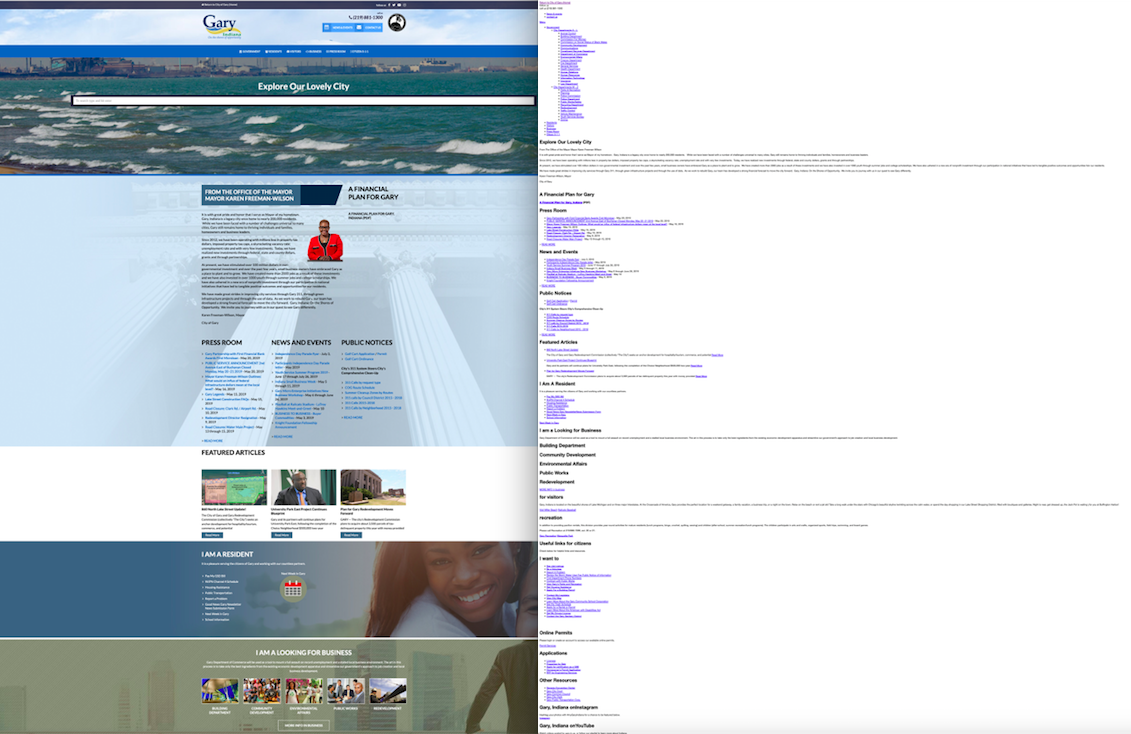
\includegraphics[scale=0.35]{figures/gary_sidebyside} \\ \vspace{.4cm}
{\bf (b)} Boilerpipe 

\includegraphics[scale=0.375]{figures/gary_bp}

\caption{The top image provides a side-by-side depiction of the entire homepage of \url{https://garyin.us/}, accessed on 05/22/2019, and complete/naive extraction of all of the text on the site. Bottom image provides the result of running \url{https://garyin.us/} through the \texttt{boilerpipe} algorithm at \url{https://boilerpipe-web.appspot.com/}.}
\label{fig:garysbs}
\end{figure}




We rely on the \texttt{boilerpipe} method described in \cite{Kohlschutter2010}, which is designed to extract blocks of substantive text from websites, and is implemented through the R package \texttt{boilerpipeR}. \texttt{boilerpipe} is a classifier that relies on both structural features, such as HTML tags, as well as text statistics such as word and sentence length to estimate whether a given portion of an HTML file is substantive. The \texttt{boilerpipe} algorithm has been widely used in the computer science and natural language processing literatures, but to our knowledge has not been previously used in political science.   The complete text extracted from the Gary, IN homepage using boilerpipe is depicted in the screenshot in the bottom row of Figure \ref{fig:garysbs}. We see that only the Mayor's message is extracted, leaving the rest of the text as boilerplate.\footnote{In the online appendix we present a replication of the topic modeling presented in the main text below in which we use a minimal HTML parser rather than \texttt{boilerpipe} to process the data. We show that without \texttt{boilerpipe}, some of the most partisan 'topics' are simply website boilerplate text. }

\subsubsection{Extracting Text from PDF, DOC, DOCX and TXT}
Other files are read in through the \texttt{readtext} R package \citep{readtext}, which is a wrapper for a set of parsers.\footnote{\texttt{readtext} determines a document's type solely through its ending---so the conversion described above is necessary.}$^{,}$\footnote{\texttt{readtext} also contains an HTML parser, but it does not eliminate boilerplate like boilerpipe.} The breakdown of all files by type is given in the online appendix. The most frequent file type besides HTML is PDF, from which we are able to extract a substantial amount of usable text. Files of type DOC, TXT, and DOCX, also occur regularly in our corpus and offer a considerable volume of textual data.

\subsection{Preprocessing}
Preprocessing is an important part of text-as-data research and choices made therein can have significant effects on the outcomes of an analysis \citep{denny2018text}. The challenge in conducting preprocessing for a comparative analysis of websites lies in the considerable variance between websites. Some of it is substantively informative and some of it is completely irrelevant. As an example of the latter, names of city officials and citizen petitioners feature frequently in city documents. The same is true for streets, locations and not least of all, the city itself. Since individual names recur at a much higher rate within a city than across the entire corpus, this would cause a topic model to cluster its topics by city. Consequently we require a tool which detects the signal in the noise and does so consistently for a discordant set of sources.

%The type of text analysis we conduct---topic modeling---requires that the words in the document be meaningful and interpretable, and does not make use of the sequence of words within a document (i.e., is a bag-of-words method). %With the exception of file type conversion and boilerplate removal, the pre-processing steps taken here should therefore not be seen as universally applicable to all analyses of government website data.

To this end, we turn to a common method in natural langauge processing---part-of-speech (POS) tagging and named entity recognition (NER). As names convey no substantive information, NER is used to detect and remove them.\footnote{We retain laws, nationalities or religious or political groups, as well as works of art (e.g., statutes).} Furthermore, we select words on the basis of their POS-tags, retaining only nouns (the modal category), verbs, and adjectives. Furthermore, we keep proper nouns that also occur as nouns---this removes names, but retains titles such as ``Police Chief'' which can appear as proper nouns if they are followed by a name. Finally, we also conduct lemmatization to reduce words to their basic form.\footnote{Lemmatization is similar to stemming, but works differently by taking grammar and surrounding words into account to identify the dictionary form of a word. } POS-tagging, NER and lemmatization are all implemented through \texttt{spacyr}. To deal with any leftover issues, we remove words with less than three characters (these are usually artifacts from improperly encoded documents and faulty or impartial optical character recognition), stopwords and non-English words (using the R package \texttt{Hunspell}).  A final and crucial step is the removal of duplicate documents, which occur very frequently on websites. In addition to their primary purpose, the previous preprocessing steps also help in stripping otherwise identical documents of information that makes them unique -- such as names and dates -- thus facilitating their deletion. %The removal of duplicate information also solves a problem posed by a recurring feature of municipal websites -- city calendars. For most days in most cities, these calendars tend to be empty, but nevertheless contain a template, which would lead to the creation of a document in our corpus. These short and repetitive -- but numerous -- texts would pose severe problems to a topic model. Our approach preserves the valuable information contained within these calendars when cities do make use of them, but removes them when they offer no substantive data.

After preprocessing, our corpus consists of 356,911 documents.  In Table \ref{tab:list} we summarize all of the steps we take in gathering and processing our data. The summary includes a brief description of the step, the software packages used, and an indicator of whether the method is implemented in our R package, \texttt{gov2text}. 

\begin{table}[ht]
    \centering
    \begin{tabular}{lrr}
        \hline
        Process & Software dependency & in \texttt{gov2text} \\
        \hline
        1. Assemble url list. & \texttt{Selenium} & no \\
        2. Collect website files. & \texttt{wget} & no \\
        3. Correct file extensions. & \texttt{wand} \citep{wand} & yes \\
        4. Discard website boilerplate. & \texttt{boilerpipeR} \citep{boilerpipeR} & yes \\
        5. Convert non-HTML files to text. & \texttt{readtext} \citep{readtext} & yes \\
        6. Lemmatize text. & \texttt{spacyr} \citep{spacyr}& yes \\
        7. Remove names. & \texttt{spacyr} & yes \\
        8. Retain nouns, verbs, adjectives. & \texttt{spacyr} & yes \\
        9. Stopword/number removal. & \texttt{quanteda} \citep{quanteda} & yes \\ 
        10. Retain only English words. & \texttt{Hunspell} \citep{hunspell} & yes \\
        11. Removal of duplicate documents. & \texttt{gov2text} & yes \\
        \hline
    \end{tabular}
    \caption{\label{tab:list} Data collection and processing pipeline. Steps to collect and prepare text for topic modeling.} 
\end{table}


%The text documents are converted to UTF-8 character encoding and then stripped of dates, punctuation, numbers, and words connected by underscores. At this point, the documents of one city still closely resemble one another in the form of boilerplate content, be it website elements (i.e. "You are here", "Home", "Directory" etc.) in HTML documents, or commonly used forms or phrases in pdf, doc and docx files. This is an issue, because this boilerplate content causes the results of analyzing this data with text analysis methods to characterize documents primarily by the cities from which they originate (through their unique boilerplate structure, e.g. a menu with certain terms repeated on every site of the domain), and not the substantive features of their contents. Boilerplate removal is a useful step in many forms of text analysis, as the analysis is focused in on text that varies above and beyond a standard template for textual content. Our solution to this problem is described in more detail in Section \ref{boilerplate}.

%The last round of preprocessing is intended to remove everything from the file that is not an English word. This step is tailored to our intention to use the text for topic modeling. The final preprocessing round includes setting every character to lowercase, as well as the removal of bullet points which frequently occur in HTML documents, extraneous whitespace, XML documents mislabeled as HTML files, and empty documents. Furthermore, some documents contain gibberish, often as a result of faulty or impartial optical character recognition applied to text that was produced through a non-machine-readable medium. To combat this problem, we employ two solutions. One, we use spellchecking, implemented through the \texttt{hunspell} R package \citep{hunspell}, to remove all non-English words.\footnote{Some of the cities, for example, Los Angeles, do contain a sizable proportion of Spanish content. The analysis of this content is beyond the scope of this paper but could be explored in future work, for example using methods of text processing that are applicable to multilingual corpora \citep{lucas2015computer}. } However, \texttt{hunspell} does not cover everything, either because some tokens are not actual words (for example artifacts from defective encoding), or because random sequences of characters just so happen to form words that exist in a dictionary (for example "eh" or "duh"). Since we rely on a bag-of-words model in which syntax does not matter, we can ameliorate these problems by removing all text except for whitespaces and the characters that appear in the English alphabet. Since a lot of the nonsensical text tends to be quite repetitive, we also delete all documents in which the proportion of unique to the total number of tokens is less than 0.15. Furthermore, \texttt{hunspell} does not spellcheck individual characters or two-character words, so we remove these token types entirely. Since these pre-processing steps reduce documents which are largely unsuitable to only a few tokens (i.e., word occurrences), we also remove all remaining documents containing less than 50 tokens. Finally, to remove words that are extremely rare (which also has the advantage of eliminating any remaining oddities) and thus add nothing substantive\footnote{Topic models essentially do not pick up on extremely rare words, so their inclusion is a waste of computational resources. Removing them in this manner is also the default preprocessing choice in the \texttt{stm} package.} to our models while increasing their computational cost, we also discard any token types that occur in only one document.

%\subsection{Boilerplate Removal}\label{boilerplate}
%As noted above, city websites contain a large amount of text that is uninformative for its actual content, and therefore a hindrance to understanding through algorithmic text analysis. This is a common issue with textual data in which informative content is embedded in technically structured documents. See, e.g., \citet{burgess2016legislative,wilkerson2015tracing} and \citet{linder2018text} for examples of boilerplate removal in the analysis of legislative text.

%\subsection*{Boilerplate Classification}
%In order to determine whether a line should be discarded, we train a classifier on a human-coded sample. We sampled 500 lines from documents in each of the following five cities: Los Angeles, CA, Indianapolis, IN, New York, NY, Shreveport, LA, and Seattle, WA. To ensure that lines which occur more frequently in these cities (sometimes hundreds of thousands of times) had a higher probability of being scrutinized by the classifier, we use sampling weights equivalent to the proportion of total lines in a city's corpus made up by each specific line type. As an example, the most common line throughout all pages of the city of Seattle consists only of the word ``total'' and occurs 103,068 times. Similarly, the line ``page'' occurs 58,833 times. Even something completely nonsensical such as ``a a'' still appears on 376 occasions. To account for the higher likelihood of some lines being part of the training set, we use inverse probability weights in training the classifier---the weight of each line in the sample is 1/[number of occurrences in the corpus].\footnote{Note that the performance of the classifier is robust to the use of these weights and only changes by about one percentage point if they are not used.}

%These 500 lines were then hand-coded as either substantively informative (210 lines) or not (290 lines). We then trained a number of different classifiers with this informativeness measure as the dependent variable. The independent variables we use are: (1) number of times the line was duplicated within the city, (2) the length of the line, in characters, (3) the number of tokens in the line, and (4) the median distance from the document midpoint to the position of the line itself. The purpose of these covariates is as follows:

\section{Partisan Language on Municipal Websites}

We illustrate the analysis of municipal website content by studying differences in website content based on the party of the mayor. As we reviewed above, the partisanship of the mayor has been found in past research to affect several features of city governance. However, \citet{gerber2011mayors} note that, due to the constraints of state and national policies, municipalities lack discretion in many domains of governance. These constraints do not apply to website contents. City governments have great discretion in composing their websites, modifying website content is low cost relative to other policy changes, and, as reviewed above, city websites provide an effective and often-used means of communication with city residents. 

%BoW methods are methods of text analysis that do not take into account the sequence or placement of words in text---just the presence and frequency of words. As noted by \cite{GrimmerStewart2013}, for most applications, bag-of-words approaches have been found to be more than sufficient. Furthermore, there is reason to believe that city government websites are a particularly `safe' case for bag-of-words methods due to their informative, manner-of-fact based language. It is extremely unlikely for these pages to feature ambiguous language such as an abundance of negation or even sarcasm.


%% latex table generated in R 3.4.4 by xtable 1.8-2 package
% Fri Aug 10 15:55:53 2018
\begin{table}[ht]
\centering
\begingroup\small
\begin{tabular}{lrr}
  \hline
Line & Substantive & Boilerplate \\ 
  \hline
have questions & 0.00 & 1.00 \\ 
  stay connected & 0.00 & 1.00 \\ 
  accident or injury & 0.00 & 1.00 \\ 
  fire damaged buildings & 0.00 & 1.00 \\ 
  gas connections & 0.00 & 1.00 \\ 
  harboring of vagrants & 0.00 & 1.00 \\ 
  roof system problem & 0.00 & 1.00 \\ 
  violation plat note & 0.00 & 1.00 \\ 
  violation setback & 0.00 & 1.00 \\ 
  violation site plan & 0.00 & 1.00 \\ 
   \hline
\end{tabular}
\endgroup
\caption{Lines (or the first 50 characters of a line) in the corpus of Anchorage, AK, with the 10 highest probabilities of being classified as boilerplate.} 
\label{tabBoilerplateIllustration}
\end{table}



To study content differences between government websites based on mayoral partisanship, we draw upon a recently-developed class model for text, the structural topic model (STM), developed by \citet{Roberts2014}. Building on the conception of ``topics'' in Latent Dirichlet Allocation, in the STM a topic is a multinomial distribution defined on the word types in the corpus dictionary. The log-odds of the topic probabilities in each document-specific multinomial distribution over topics are drawn from a multivariate normal distribution in which the topic-specific means are determined by a linear regression function that associates document-attributed covariates with topics. For example, in the context of municipal website content, the structural topic model can be used to estimate a regression coefficient that defines the linear relationship between the log-odds of the municipality's population and the log-odds of each topic. For our primary empirical investigation, the STM provides a tool to estimate the relationship between the party of the city's mayor and the prevalence of each topic. We also include the municipality's population and median income as covariates. Further details on and results from our STM specification can be found in the online appendix.


\subsubsection{Structural topic model results}


The results are shown in Table \ref{tabSTMtopwords60}. First, it is notable that the 95\% credible interval includes zero in only seven of the sixty topics, indicating that the topics discussed on city websites varies systematically with the partisanship of the mayor. Many of the topics associated with Democrats fit with what we understand to be national party priorities. Topic \textbf{52}, on affordable housing, clearly resonates with the Democratic party's appeal to low-income voters. Topic {\bf 6} ('race', 'islander', 'census, 'female') covers racial and gender identity issues. Similarly, employee rights and benefits are represented in topics \textbf{10} and \textbf{29}. Democrats also exhibit a strong preference for words related to public finances, such as Topic \textbf{58} ('budget', 'revenue', 'expenditure'), Topic {\bf 45} ('asset', 'actuarial', 'liability', 'financial'), Topic \textbf{35} ('bond', 'obligation', 'proceeds') as well as Topic \textbf{55} ('taxable', 'deed', 'value'). We suspect that the association of Democratic mayors with finance-related terms is indicative of a greater willingness to emphasize the city's efforts to raise and spend money, and take credit for those efforts (e.g., the Gary, IN example in Figure \ref{fig:garymayor}). This finding is consistent with \cite{Einstein2015}, who show that Democratic mayors tend to favor greater spending. A second, consistent Democratic focus appears to be law enforcement: The most Democratic topic, \textbf{59} ('burglary', 'robbery', 'theft', 'homicide') is clearly focused on crime. On the one hand, Democratic partisans have a more negative perception of the police, rating it considerably more negatively on the appropriate use of force and the equal treatment of minorities \citep{Brown2017}. On the other hand, the literature has also shown that cities with a higher Democratic vote share spend more on law enforcement, even after controlling for crime \citep{Einstein2015}. 

City websites with Republican mayors, meanwhile, exhibit a pronounced focus on the essential functions of government. Basic utilities such as energy (Topic \textbf{20}), fire protection (Topic \textbf{51}), vaccination (Topic \textbf{2}),  and sanitation (Topic \textbf{47}), are prevalent among cities with Republican mayors. These basic service topics cannot be found among topics prevalent in cities with Democratic mayors. Similarly, zoning issues figure prominently in the set of republican topic (Topic \textbf{19}), which fits with the findings of \citet{sorens2018effects} that Republicans are more supportive of restrictive residential zoning rules. The Democratic topics also include one that is somewhat focused on zoning, Topic {\bf 39} ('downtown', 'mixed', 'density'), but emphasizes mixed-use zoning---a loosening of conventional single-use zoning rules.



%Interestingly enough, Democrats also `own' the topic related to law enforcement, which might be somewhat unexpected given Republicans' usual focus on law and order \citep{gerber2011mayors}. However, this kind of finding is not entirely without precedent in the literature (see \citep{Einstein2015}). Similar to the informed dirichlet model, the structural topic model also finds the emphasis on construction and infrastructure by Republicans - in table \ref{tabSTMINRep}, topics 2, 7 and 8 clearly focus on these issues.\footnote{The first Republican topic in Indiana (library, stream, obj, etc.) is likely an artifact from incorrectly converted HTML, and since it presumably only happens only in one Republican city, the topic is classified as very Republican.}

%When comparing Indiana to Louisiana, it appears that the Democratic emphasis on law enforcement is robust. Furthermore, as with the fightin' words approach, some smaller degree of focus on money (see topic 1) is still evident. For Republicans, topics 2 to 4 seem to be, once again about infrastructure and utilities, pointing to a certain degree of robustness in these results, as well as the emergence of a trend. The results produced by the structural topic model are not flawless, but the two parties do seem to have somewhat consistent themes on which they focus on in both states. Furthermore, in comparison to the fightin' words approach, the ability of the structural topic model to form coherent topics is quite evident and helpful in the interpretation of the results.

%An ostensibly intuitive solution to topics clustering into cities in LDA is to include dummies for the cities in a statistical model of topics. This is facilitated by the structural topic model, which uses document metadata t to account for variation in topics \citep{Roberts2014}. However, figure \ref{stm_results} shows that if anything, the STM exacerbates the problem. Here, we plot the \textit{p-values} of the coefficients for each city as well as the party variable across each topic. Under normal circumstances, plotting the p-values, as opposed to the fitted values, does not make much sense, but here it serves a diagnostic purpose. The plot shows that the party variable is never statistically significant at any conceivable level of confidence, nor is it even close to. Interestingly the same is true for a number of the cities as well. The topics cluster heavily into only about half of the cities, which does not present an improvement over LDA at all.

%Partisan top words - stm Louisiana -- Rep
%% latex table generated in R 3.4.2 by xtable 1.8-2 package
% Mon Nov 13 15:36:58 2017
\begin{table}[ht]
\centering
\begin{tabular}{llllll}
  \hline
0.024 & 0.019 & 0.019 & 0.016 & 0.016 & 0.016 \\ 
  \hline
motion & plan & inc & request & council & \cellcolor{red!25} traffic \\ 
  second & \cellcolor{red!25} zone & electr & board & citi & amp \\ 
  made & applic & build & member & ordin & vehicl \\ 
  approv & \cellcolor{red!25} properti & construct & servic & common & stop \\ 
  mayor & approv & home & \cellcolor{red!25} street & councilor & sign \\ 
  present & sign & street & approv & amend & \cellcolor{red!25} road \\ 
  state & \cellcolor{red!25} site & meridian & purchas & resolut & block \\ 
  will & locat & servic & citi & adopt & signal \\ 
  citi & commiss & west & move & wherea & \cellcolor{red!25} street \\ 
  council & file & main & good & approv & driver \\ 
   \hline
\end{tabular}
%\caption{Top Republican topics and words (Indiana), according to STM. 
%The words are the top words for the most Democratic/Republican topic, determined
%by the size (and significance) of the coefficient (see table header) of the party covariate.} 
\label{tabSTMINRep}
\end{table}

 %\ref{tabSTMINRep}

%Partisan top words - stm Louisiana -- Dem
%% latex table generated in R 3.4.3 by xtable 1.8-2 package
% Tue Dec 26 20:59:22 2017
\begin{table}[ht]
\centering
\scriptsize
\begin{tabular}{llllll}
  \hline
-0.027 & -0.022 & -0.016 & -0.011 & -0.011 & -0.01 \\ 
  \hline
city & school & downtown & city & \cellcolor{blue!25}trash & \cellcolor{blue!25}housing \\ 
  ordinance & community & business & department & city & property \\ 
  approve & program & project & mayor & \cellcolor{blue!25}waste & program \\ 
  resolution & student & city & police & day & \cellcolor{blue!25}fund \\ 
  property & \cellcolor{blue!25}education & \cellcolor{blue!25}development & officer & \cellcolor{blue!25}recycle & home \\ 
  purchase & \cellcolor{blue!25}university & new & public & street & city \\ 
  area & national & center & citizen & collection & project \\ 
  department & award & \cellcolor{blue!25}economic & work & resident & neighborhood \\ 
  contract & high & company & safety & \cellcolor{blue!25}recycling & \cellcolor{blue!25}grant \\ 
  service & year & community & resident & snow & unit \\ 
   \hline
\end{tabular}
\caption{Top Democratic topics and words}%\caption{Top Democratic topics and words (Indiana), according to STM. 
%The words are the top words for the most Democratic/Republican topic, determined
%by the size (and significance) of the coefficient (see table header) of the party covariate.} 
\label{tabSTMINDem}
\end{table}

 %\ref{tabSTMLADem}

%Partisan top words - stm Louisiana -- Rep
%% latex table generated in R 3.4.3 by xtable 1.8-2 package
% Tue Dec 26 15:50:18 2017
\begin{table}[ht]
\centering
\begin{tabular}{llllllll}
  \hline
0.071 & 0.054 & 0.054 & 0.034 & 0.033 & 0.024 & 0.023 & 0.02 \\ 
  \hline
event & ordinance & water & street & say & city & city & mayor \\ 
  information & department & emergency & traffic & can & business & meeting & city \\ 
  show & summary & city & parking & make & new & council & parish \\ 
  park & amount & resident & lane & get & mayor & commission & town \\ 
  music & bid & storm & project & take & development & plan & office \\ 
  food & city & weather & work & people & economic & member & hall \\ 
  visit & public & waste & bike & work & million & public & contact \\ 
  weekend & police & system & downtown & need & continue & board & day \\ 
  festival & approve & power & public & city & work & committee & official \\ 
  begin & inc & service & bicycle & help & local & planning & state \\ 
   \hline
\end{tabular}
\caption{Top Republican topics and words (Louisiana), according to STM. 
The words are the top words for the most Democratic/Republican topic, determined
by the size (and significance) of the coefficient (see table header) of the party covariate.} 
\label{tabSTMLARep}
\end{table}

 %\ref{tabSTMLARep}

%Partisan top words - stm Louisiana -- Dem
%% latex table generated in R 3.4.3 by xtable 1.8-2 package
% Mon Dec 25 01:20:56 2017
\begin{table}[ht]
\centering
\begin{tabular}{llllllll}
  \hline
-0.044 & -0.04 & -0.021 & -0.019 & -0.016 & -0.012 & -0.011 & -0.01 \\ 
  \hline
owner & provide & victim & application & employee & city & revenue & community \\ 
  applicant & otherwise & crime & motion & policy & ordinance & fund & neighborhood \\ 
  new & respect & violence & second & city & whereas & tax & district \\ 
  application & thereto & arrest & street & report & bond & budget & police \\ 
  per & city & domestic & favor & department & resolution & million & public \\ 
  exist & authorize & officer & retention & audit & code & total & meeting \\ 
  build & ordinance & suspect & john & review & provide & year & engagement \\ 
  proposal & amend & report & arc & management & shall & general & crime \\ 
  receive & district & child & window & procedure & provision & service & officer \\ 
  construction & locate & police & heather & work & fund & forecast & department \\ 
   \hline
\end{tabular}
\caption{Top Democratic topics and words (Louisiana), according to STM. 
The words are the top words for the most Democratic/Republican topic, determined
by the size (and significance) of the coefficient (see table header) of the party covariate.} 
\label{tabSTMLADem}
\end{table}

 %\ref{tabSTMLADem}

%\subsubsection{Prediction with SVM}
%An alternative approach to the problem is to ignore topics entirely and go straight to predicting documents that are much more likely to be included on websites belonging to one or the other party. Classic machine learning techniques such as Naive Bayes, Linear Discriminant Analysis, or SVM should be expected to fare well in this context. Here, we rely on SVM, implemented with the SciKitLearn package in Python.\footnote{We also implemented SVM in R through the packages kernlab and e1071 in R. However, neither of these provide a regularized version of SVM (NOTE: at least that is what I am gathering from the stack overflow error), which prevents us from using all of the features contained in our data. Instead, we ranked the features according to tf-idf and selected the top 5000. These methods are also quite slow, and provide a maximum accuracy of 82\% in five-fold cross-validation.} A grid search reveals the tf-idf representation of the document-term matrix to be better than pure word counts, unigrams to be superior to bi-grams, the application of an L2 penalty to be preferable to either L1 or elasticnet, and an alpha (a constant to multiply with the regularization parameter C) of 0.0005 to lead to the best results. Applying five-fold cross-validation to the (tf-idf) document-term matrix with the dimensions 16011x35000 leads to an average accuracy of 89\%.\footnote{Other methods used: Elastic-net in the glmnet package in R. Accuracy is 0.6924795 for in-sample prediction, so not worth bothering with.}

%However, \cite{Monroe2008} advise against using these types of methods in this context because they get the data generation process backward: Our theory assumes that party leads to variation in writing, and yet we rely on the documents to predict party, in spite of the fact that we actually have perfect knowledge of it.



%Heatmaps
%\begin{figure}[htp]
%    \centering % Using \begin{figure*} makes the figure take up the entire width of the page
%    \caption{Word-topic probabilities for topics with big partisan differences, across documents (Indiana).}
%    \label{heatmaps_weights}
%    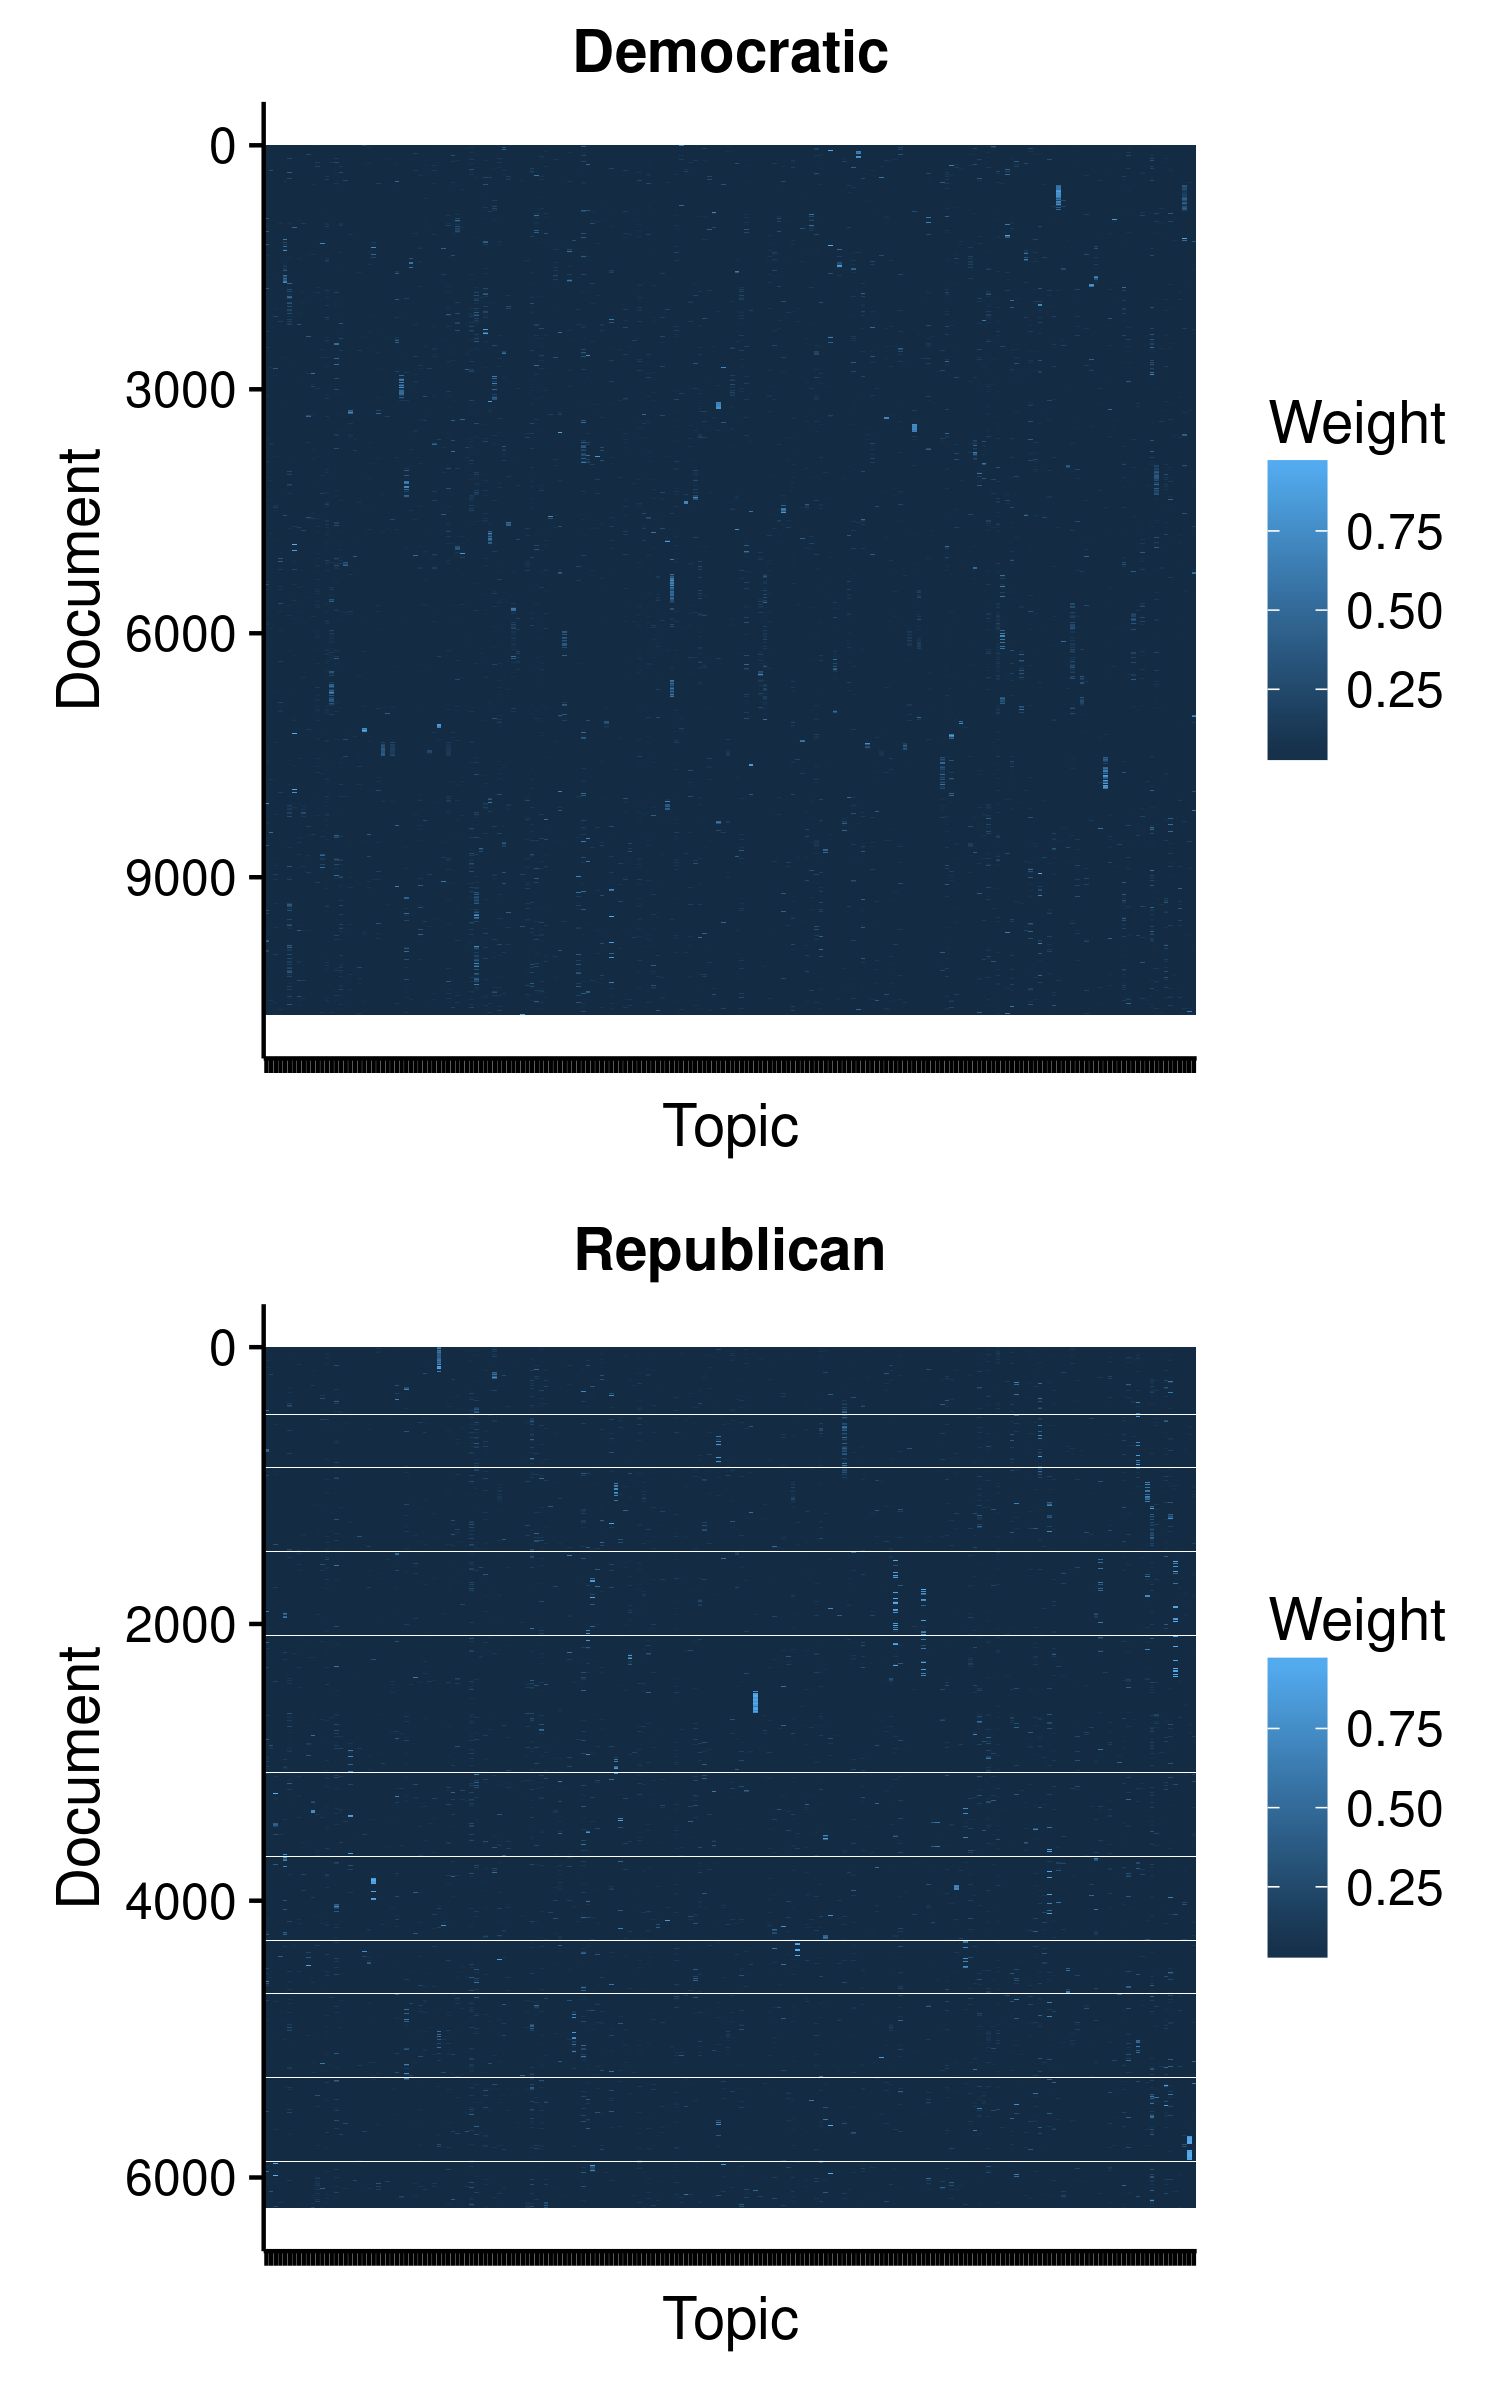
\includegraphics[width=0.8\linewidth]{figures/heatmaps_weights_IN.png}
%\end{figure}



%US map
%\begin{figure}[htp]
  %  \centering % Using \begin{figure*} makes the figure take up the entire width of the page
    %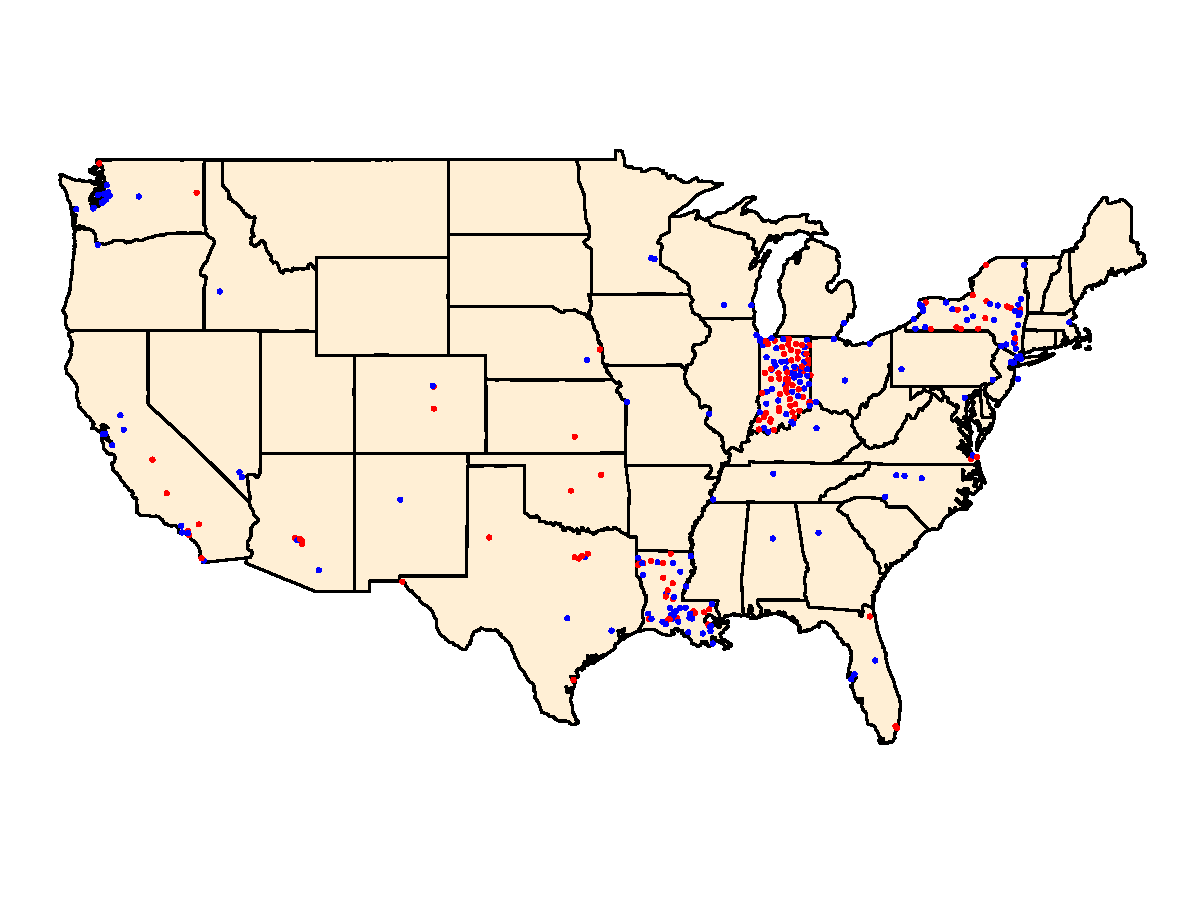
\includegraphics[width=\linewidth]{figures/us_map.pdf} \vspace{-2cm}
       % \caption{Map of the cities in the corpus in the contiguous U.S. The corpus also includes Alaska. In the analysis, only cities in California, Indiana, Louisiana, New York, Texas and Washington are used. The colors represent the partisanship of the mayor (blue corresponding to Democrats and red to Republicans).}
    %\label{us_map}
%\end{figure}

%stm results
%\begin{figure}[htp]
%    \centering % Using \begin{figure*} makes the figure take up the entire width of the page
%    \caption{Results from a structural topic model, displayed as the p-values for each variable for each topic. This would normally be somewhat nonsensical, but here it illustrates why the model does not work.}
%    \label{stm_results}
%%    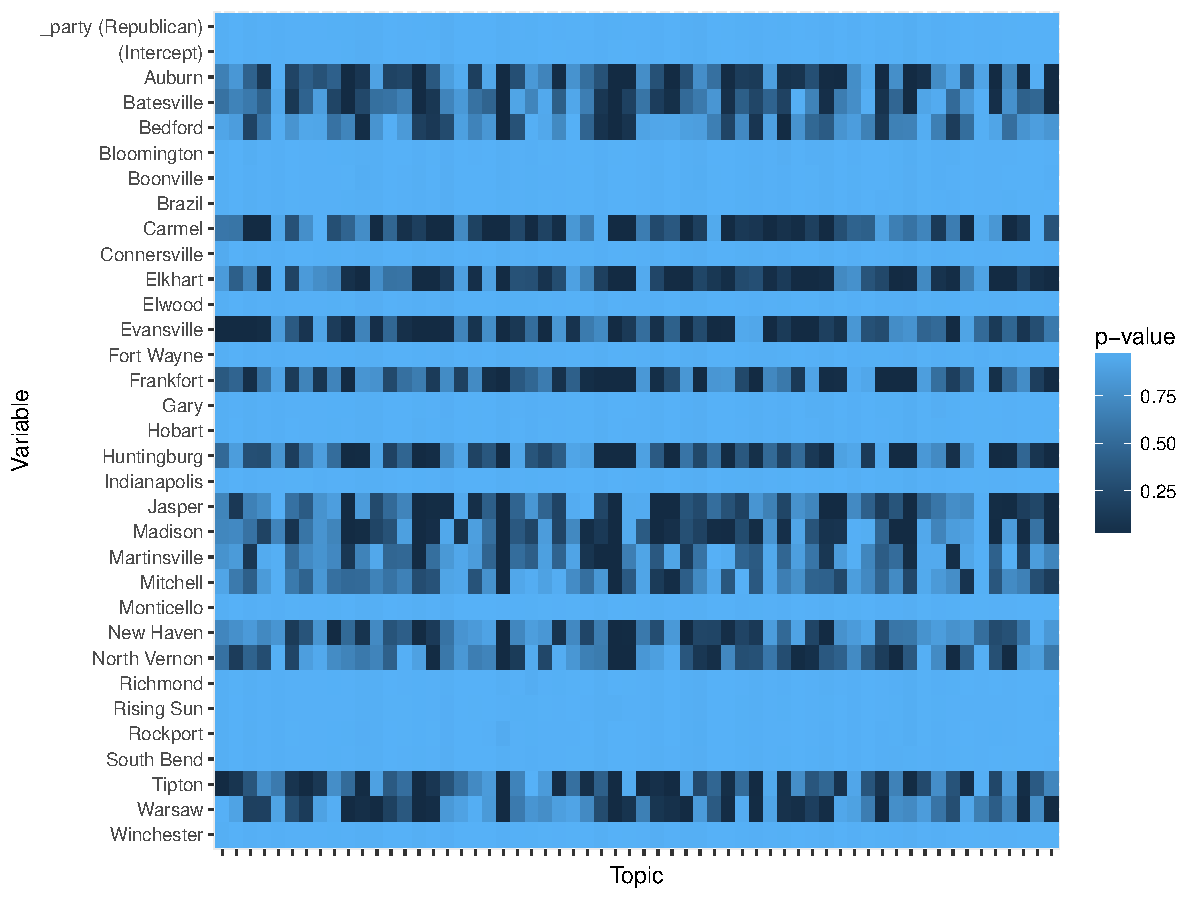
\includegraphics[width=1.1\linewidth]{figures/stm_results.pdf}
%\end{figure}



%Partisan top words - topic model Indiana
%% latex table generated in R 3.4.1 by xtable 1.8-2 package
% Fri Oct 20 13:14:52 2017
\begin{table}[ht]
\centering
\begingroup\fontsize{9pt}{10pt}\selectfont
\begin{tabular}{lrlr}
  \hline
Word (D) & Instances (D) & Word (R) & Instances (R) \\ 
  \hline
city & 42493 & will & 53761 \\ 
  said & 40480 & city & 36210 \\ 
  county & 39209 & street & 21207 \\ 
  proposal & 29019 & board & 19496 \\ 
  public & 27070 & water & 18637 \\ 
  council & 23492 & plan & 18241 \\ 
  shall & 23162 & public & 14327 \\ 
  department & 22926 & use & 13233 \\ 
  services & 22703 & information & 13062 \\ 
  fund & 21661 & development & 12916 \\ 
  will & 20697 & department & 11554 \\ 
  new & 19000 & area & 11270 \\ 
  stated & 18794 & shall & 11247 \\ 
  project & 18538 & fire & 10861 \\ 
  property & 18378 & can & 10748 \\ 
  budget & 16631 & must & 10633 \\ 
  community & 16236 & park & 10493 \\ 
  asked & 16231 & building & 10356 \\ 
  tax & 14549 & motion & 10168 \\ 
  board & 14363 & ordinance & 9625 \\ 
  state & 13964 & request & 9512 \\ 
  office & 13818 & council & 9098 \\ 
  program & 13536 & community & 9072 \\ 
  year & 13376 & meeting & 8990 \\ 
  service & 13312 & ave & 8555 \\ 
  provide & 13138 & service & 8040 \\ 
  one & 13066 & construction & 7999 \\ 
  section & 12669 & one & 7885 \\ 
  work & 11986 & property & 7741 \\ 
  information & 11886 & also & 7492 \\ 
  development & 11854 & per & 7442 \\ 
  committee & 11802 & required & 7407 \\ 
  district & 11584 & home & 7334 \\ 
  time & 11466 & center & 7316 \\ 
  total & 10965 & made & 7301 \\ 
  general & 10731 & site & 7279 \\ 
  parks & 10704 & business & 7222 \\ 
  system & 10668 & time & 7157 \\ 
  digest & 10481 & services & 7140 \\ 
  police & 10474 & housing & 7111 \\ 
  management & 10433 & new & 7006 \\ 
  park & 10356 & within & 6910 \\ 
  also & 10112 & date & 6818 \\ 
  division & 9964 & year & 6768 \\ 
  street & 9853 & following & 6754 \\ 
  resolution & 9768 & road & 6629 \\ 
  contract & 9763 & member & 6450 \\ 
  ordinance & 9456 & inc & 6367 \\ 
  safety & 9362 & number & 6360 \\ 
  code & 9342 & day & 6254 \\ 
   \hline
\end{tabular}
\endgroup
\caption{Top 50 Democratic and Republican words (Indiana), according to LDA. 
             Topic ownership is determined by the ratio of Democratic to Republican tokens in 
             it (both weighted by the total number of tokens per party). The instances of each 
             token type are then summed across all topics owned by the party.} 
\label{tabLDAIN}
\end{table}

 %\ref{tabFightinIN}

%Partisan top words - topic model Louisiana
%% latex table generated in R 3.4.1 by xtable 1.8-2 package
% Fri Oct 20 12:46:14 2017
\begin{table}[ht]
\centering
\begingroup\fontsize{9pt}{10pt}\selectfont
\begin{tabular}{lrlr}
  \hline
Word (D) & Instances (D) & Word (R) & Instances (R) \\ 
  \hline
city & 19306 & city & 9930 \\ 
  stream & 13397 & ordinance & 4413 \\ 
  new & 13001 & information & 3756 \\ 
  obj & 10440 & council & 3422 \\ 
  otherwise & 8271 & said & 3301 \\ 
  street & 7990 & plan & 3194 \\ 
  provide & 7647 & department & 2991 \\ 
  district & 7449 & state & 2598 \\ 
  property & 7031 & public & 2594 \\ 
  public & 6864 & meeting & 2392 \\ 
  shall & 6750 & mayor & 2258 \\ 
  respect & 6698 & one & 2166 \\ 
  water & 6085 & application & 2105 \\ 
  thereto & 5686 & development & 2017 \\ 
  development & 5124 & parish & 1809 \\ 
  use & 5086 & can & 1807 \\ 
  ordinance & 4963 & new & 1807 \\ 
  business & 4763 & water & 1780 \\ 
  department & 4757 & program & 1691 \\ 
  community & 4705 & project & 1674 \\ 
  authorizing & 4440 & time & 1648 \\ 
  located & 4315 & code & 1641 \\ 
  mayor & 4266 & year & 1560 \\ 
  length & 4215 & date & 1556 \\ 
  project & 3918 & number & 1548 \\ 
  section & 3863 & name & 1516 \\ 
  service & 3831 & street & 1504 \\ 
  councilman & 3824 & motion & 1500 \\ 
  services & 3782 & day & 1483 \\ 
  zoning & 3771 & park & 1471 \\ 
  parish & 3731 & home & 1469 \\ 
  providing & 3641 & address & 1415 \\ 
  one & 3636 & office & 1408 \\ 
  system & 3617 & amount & 1392 \\ 
  building & 3607 & ave & 1384 \\ 
  can & 3557 & budget & 1382 \\ 
  code & 3532 & please & 1375 \\ 
  office & 3305 & community & 1334 \\ 
  drive & 3223 & area & 1326 \\ 
  work & 3171 & contact & 1319 \\ 
  permit & 3165 & emergency & 1308 \\ 
  following & 3153 & summary & 1282 \\ 
  within & 3123 & also & 1271 \\ 
  must & 3088 & make & 1265 \\ 
  plan & 3064 & two & 1224 \\ 
  neighborhood & 3048 & work & 1213 \\ 
  construction & 3016 & fire & 1184 \\ 
  chapter & 2973 & bid & 1134 \\ 
  ordinances & 2885 & planning & 1124 \\ 
  fire & 2878 & people & 1108 \\ 
   \hline
\end{tabular}
\endgroup
\caption{Top 50 Democratic and Republican words (Louisiana), according to LDA. 
             Topic ownership is determined by the ratio of Democratic to Republican tokens in 
             it (both weighted by the total number of tokens per party). The instances of each 
             token type are then summed across all topics owned by the party.} 
\label{tabLDALA}
\end{table}

 %tabLDALA

%Partisan top words - stm Indiana
%% latex table generated in R 3.4.2 by xtable 1.8-2 package
% Tue Nov  7 21:46:14 2017
\begin{table}[ht]
\centering
\caption{Top 50 Democratic and Republican words (Indiana), according to STM. 
             The words are the top words for the most Democratic/Republican topic, determined
             by the size (and significance) of the coefficient of the party covariate.} 
\label{tabSTMIN}
\begingroup\footnotesize
\begin{tabular}{ccr|ccr}
  \toprule 
 \multicolumn{3}{c}{\textbf{Democratic}} & \multicolumn{3}{c}{\textbf{Republican}} \\
 \cmidrule(l){1-3} \cmidrule(l){4-6}
  Topic & Coefficient & Word & Topic & Coefficient & Word \\
 \midrule 
   59 & -0.026 & fort &   28 & 0.024 & motion \\ 
    59 & -0.026 & citi &   28 & 0.024 & second \\ 
    59 & -0.026 & ordin &   28 & 0.024 & made \\ 
    59 & -0.026 & approv &   28 & 0.024 & approv \\ 
    59 & -0.026 & purchas &   28 & 0.024 & mayor \\ 
    59 & -0.026 & depart &   28 & 0.024 & present \\ 
    59 & -0.026 & properti &   28 & 0.024 & state \\ 
    59 & -0.026 & will &   28 & 0.024 & will \\ 
    59 & -0.026 & resolut &   28 & 0.024 & citi \\ 
    59 & -0.026 & contract &   28 & 0.024 & council \\ 
   \cmidrule(l){1-3} \cmidrule(l){4-6}
  50 & -0.019 & propos &   11 & 0.019 & plan \\ 
    50 & -0.019 & author &   11 & 0.019 & zone \\ 
    50 & -0.019 & district &   11 & 0.019 & applic \\ 
    50 & -0.019 & street &   11 & 0.019 & properti \\ 
    50 & -0.019 & public &   11 & 0.019 & approv \\ 
    50 & -0.019 & control &   11 & 0.019 & sign \\ 
    50 & -0.019 & amend &   11 & 0.019 & site \\ 
    50 & -0.019 & intersect &   11 & 0.019 & locat \\ 
    50 & -0.019 & counti &   11 & 0.019 & commiss \\ 
    50 & -0.019 & committe &   11 & 0.019 & file \\ 
   \cmidrule(l){1-3} \cmidrule(l){4-6}
  42 & -0.018 & said &    2 & 0.019 & inc \\ 
    42 & -0.018 & ask &    2 & 0.019 & electr \\ 
    42 & -0.018 & state &    2 & 0.019 & build \\ 
    42 & -0.018 & will &    2 & 0.019 & construct \\ 
    42 & -0.018 & chair &    2 & 0.019 & home \\ 
    42 & -0.018 & propos &    2 & 0.019 & street \\ 
    42 & -0.018 & year &    2 & 0.019 & meridian \\ 
    42 & -0.018 & move &    2 & 0.019 & servic \\ 
    42 & -0.018 & need &    2 & 0.019 & west \\ 
    42 & -0.018 & council &    2 & 0.019 & main \\ 
   \cmidrule(l){1-3} \cmidrule(l){4-6}
  16 & -0.018 & prosecutor &   27 & 0.016 & request \\ 
    16 & -0.018 & charg &   27 & 0.016 & board \\ 
    16 & -0.018 & feloni &   27 & 0.016 & member \\ 
    16 & -0.018 & counti &   27 & 0.016 & servic \\ 
    16 & -0.018 & case &   27 & 0.016 & street \\ 
    16 & -0.018 & crime &   27 & 0.016 & approv \\ 
    16 & -0.018 & crimin &   27 & 0.016 & purchas \\ 
    16 & -0.018 & offic &   27 & 0.016 & citi \\ 
    16 & -0.018 & victim &   27 & 0.016 & move \\ 
    16 & -0.018 & sentenc &   27 & 0.016 & good \\ 
   \cmidrule(l){1-3} \cmidrule(l){4-6}
  13 & -0.018 & digest &   35 & 0.016 & council \\ 
    13 & -0.018 & introduc &   35 & 0.016 & citi \\ 
    13 & -0.018 & author &   35 & 0.016 & ordin \\ 
    13 & -0.018 & counti &   35 & 0.016 & common \\ 
    13 & -0.018 & appoint &   35 & 0.016 & councilor \\ 
    13 & -0.018 & board &   35 & 0.016 & amend \\ 
    13 & -0.018 & approv &   35 & 0.016 & resolut \\ 
    13 & -0.018 & district &   35 & 0.016 & adopt \\ 
    13 & -0.018 & fund &   35 & 0.016 & wherea \\ 
    13 & -0.018 & street &   35 & 0.016 & approv \\ 
   \bottomrule 
\end{tabular}
\endgroup
\end{table}

 %\ref{tabSTMLA}

%Partisan top words - stm Louisiana
%% latex table generated in R 3.4.2 by xtable 1.8-2 package
% Sun Oct 29 16:12:17 2017
\begin{table}[ht]
\centering
\begingroup\fontsize{9pt}{10pt}\selectfont
\begin{tabular}{rrlrrl}
  \hline
demTopic & demTopicCoeff & Democratic & repTopic & repTopicCoeff & Republican \\ 
  \hline
   1 & -0.171 & stream &   49 & 0.095 & event \\ 
     1 & -0.171 & obj &   49 & 0.095 & music \\ 
     1 & -0.171 & interpol &   49 & 0.095 & church \\ 
     1 & -0.171 & baa &   49 & 0.095 & inform \\ 
     1 & -0.171 & matrix &   49 & 0.095 & show \\ 
     1 & -0.171 & metadata &   49 & 0.095 & park \\ 
     1 & -0.171 & hum &   49 & 0.095 & market \\ 
     1 & -0.171 & gym &   49 & 0.095 & visit \\ 
     1 & -0.171 & rid &   49 & 0.095 & year \\ 
     1 & -0.171 & yep &   49 & 0.095 & featur \\ 
    15 & -0.045 & length &   13 & 0.093 & said \\ 
    15 & -0.045 & root &   13 & 0.093 & work \\ 
    15 & -0.045 & predictor &   13 & 0.093 & citi \\ 
    15 & -0.045 & eye &   13 & 0.093 & depart \\ 
    15 & -0.045 & word &   13 & 0.093 & airport \\ 
    15 & -0.045 & acrobat &   13 & 0.093 & code \\ 
    15 & -0.045 & adob &   13 & 0.093 & offici \\ 
    15 & -0.045 & ash &   13 & 0.093 & resid \\ 
    15 & -0.045 & rang &   13 & 0.093 & mayor \\ 
    15 & -0.045 & vet &   13 & 0.093 & continu \\ 
    57 & -0.044 & otherwis &   56 & 0.064 & ordin \\ 
    57 & -0.044 & provid &   56 & 0.064 & summari \\ 
    57 & -0.044 & respect &   56 & 0.064 & amount \\ 
    57 & -0.044 & thereto &   56 & 0.064 & citi \\ 
    57 & -0.044 & citi &   56 & 0.064 & bid \\ 
    57 & -0.044 & author &   56 & 0.064 & depart \\ 
    57 & -0.044 & ordin &   56 & 0.064 & motion \\ 
    57 & -0.044 & amend &   56 & 0.064 & approv \\ 
    57 & -0.044 & district &   56 & 0.064 & public \\ 
    57 & -0.044 & locat &   56 & 0.064 & contract \\ 
    41 & -0.017 & pdf &   12 & 0.049 & flood \\ 
    41 & -0.017 & content &   12 & 0.049 & emerg \\ 
    41 & -0.017 & type &   12 & 0.049 & storm \\ 
    41 & -0.017 & width &   12 & 0.049 & disast \\ 
    41 & -0.017 & text &   12 & 0.049 & weather \\ 
    41 & -0.017 & resourc &   12 & 0.049 & hurrican \\ 
    41 & -0.017 & parent &   12 & 0.049 & can \\ 
    41 & -0.017 & filter &   12 & 0.049 & area \\ 
    41 & -0.017 & font &   12 & 0.049 & busi \\ 
    41 & -0.017 & page &   12 & 0.049 & inform \\ 
     5 & -0.017 & polic &    3 & 0.022 & councilman \\ 
     5 & -0.017 & crime &    3 & 0.022 & want \\ 
     5 & -0.017 & offic &    3 & 0.022 & said \\ 
     5 & -0.017 & investig &    3 & 0.022 & just \\ 
     5 & -0.017 & arrest &    3 & 0.022 & know \\ 
     5 & -0.017 & suspect &    3 & 0.022 & get \\ 
     5 & -0.017 & victim &    3 & 0.022 & like \\ 
     5 & -0.017 & report &    3 & 0.022 & citi \\ 
     5 & -0.017 & block &    3 & 0.022 & can \\ 
     5 & -0.017 & vehicl &    3 & 0.022 & come \\ 
   \hline
\end{tabular}
\endgroup
\caption{Top 50 Democratic and Republican words (Louisiana), according to STM. 
             The words are the top words for the most Democratic/Republican topic, determined
             by the size (and significance) of the coefficient of the party covariate.} 
\label{tabSTMLA}
\end{table}

 %\ref{tabSTMLA}


%Some basic descriptive statistics of documents by party
%% latex table generated in R 3.4.1 by xtable 1.8-2 package
% Fri Oct 20 13:41:38 2017
\begin{table}[ht]
\centering
\begin{tabular}{rrr}
  \hline
 & Democratic & Republican \\ 
  \hline
Cities & 15 & 17 \\ 
  Documents & 10257 & 5859 \\ 
  Tokens & 6101752 & 2310072 \\ 
  Token assignments & 6006202 & 2259362 \\ 
  Topics & 103 & 97 \\ 
   \hline
\end{tabular}
\caption{Descriptive statistics for Indiana. ``Tokens'' describes the number
             of words in each party's documents, ``token assignments'' the tokens assigned
             to each party in the topic model depending on the ratio of Democratic to Republican 
             tokens in it (both weighted by the total number of tokens per party).} 
\label{tabDescriptiveIN}
\end{table}



%Some basic descriptive statistics of documents by party
%% latex table generated in R 3.4.1 by xtable 1.8-2 package
% Fri Oct 20 13:53:50 2017
\begin{table}[ht]
\centering
\begin{tabular}{rrr}
  \hline
 & Democratic & Republican \\ 
  \hline
Cities & 11 & 7 \\ 
  Documents & 6287 & 1327 \\ 
  Tokens & 1955198 & 322915 \\ 
  Token assignments & 1789373 & 314628 \\ 
  Topics & 143 & 57 \\ 
   \hline
\end{tabular}
\caption{Descriptive statistics for Louisiana. ``Tokens'' describes the number
             of words in each party's documents, ``token assignments'' the tokens assigned
             to each party in the topic model depending on the ratio of Democratic to Republican 
             tokens in it (both weighted by the total number of tokens per party).} 
\label{tabDescriptiveLA}
\end{table}



%fightin words results
%\begin{figure}[htp]
%    \centering % Using \begin{figure*} makes the figure take up the entire width of the page
%    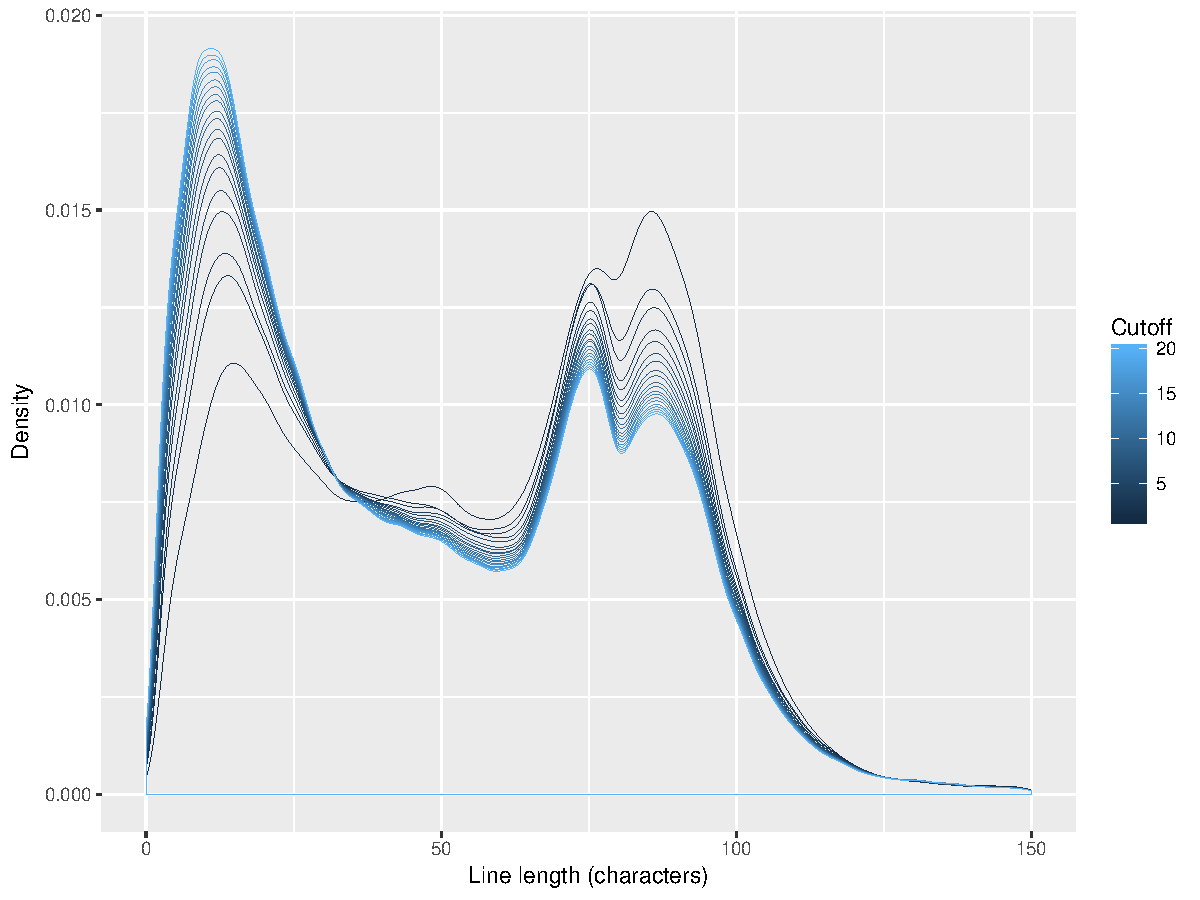
\includegraphics[width=\linewidth]{figures/linesCutoffIN.pdf}
%        \caption{Total number of lines retained at a given threshold for removing duplicated lines. For example, at x = 10, all lines occurring more than 10 times within a city's documents are removed.}
%    \label{linesCutoff}
%\end{figure}


%\section{Ground truth test}
%In the realm of public administration, the notion that the partisan leaning of mayors might have an effect on how they run their cities is still frowned upon to some extent. Perceived more as managers than politicians, they have been portrayed as the last bastion of non-partisanship in America, and in many cases, also style themselves that way \citep{Dovere2018}. However, the aspirations some mayors have shown towards higher offices - in some cases, even the presidency - reveal that they are not quite as above the fray as some may believe them to be. One of the most vicious and blatantly partisan cleavages in current U.S. politics - the debate surrounding sanctuary cities - has seen mayors in a central role. Research into local politics has shown that partisan elections consistently have greater turnout \citep{Schaffner2001}. When voters are denied this cue, they make use of other, and considerably more irrational heuristics, such as name, gender, or occupation of the contenders. Consequently, it only makes sense for any office-seeking politician to emphasize their partisanship. Finally, decades of research in political psychology have consistently shown that no matter how hard we try, humans are simply incapable of escaping our partisan biases, a finding that is especially pronounced among elites \citep{Hatemi2011}.
%
%In an effort to underline this fact and remove any doubt about the fact that the partisanship of mayors colors their decision-making, we conduct a ground truth test between our main corpus - the websites of cities - and a second, decidedly more partisan set of texts: the campaign websites of these mayors. As noted above, partisanship has been shown to be a powerful driving force even in local politics, and mayors are incentivized to exploit it. Consequently, they are very likely to emphasize conservative/liberal values on this platform. If there is a greater correlation in word use between the cities managed by a party and the campaign websites of its mayors than with those of the other party, evidence for the partisanship of city websites can be established.
%
%Using the same methods as described for our main corpus, we have gathered these sites and then concatenated all of the documents belonging to mayors of the two parties into one ground truth document each. We do the same for the city documents, and then compare the four document collections using cosine similarity. This measure is the cosine between the angle of two vectors, in this case, the frequencies of all words in the two vocabularies. Compared to a simple Euclidean distance, this has the advantage of accounting for the fact that the two corpora being compared are not necessarily of the same length. The cosine measure between two documents ranges between 0 and 1, 0 signifying absolutely no correlation, and 1 perfect overlap. Figure \ref{groundtruth} shows the result of this test. The expectation is for a greater similarity between Republican cities and the Republican ground truth than Republican cities and Democratic ground truth - and vice versa. At present, however, this does not appear to be the case, presumably because the Republican ground truth consists of 8 documents, and the Democratic one of 290.

%ground truth test
%\begin{figure}[htp]
%    \centering % Using \begin{figure*} makes the figure take up the entire width of the page
%    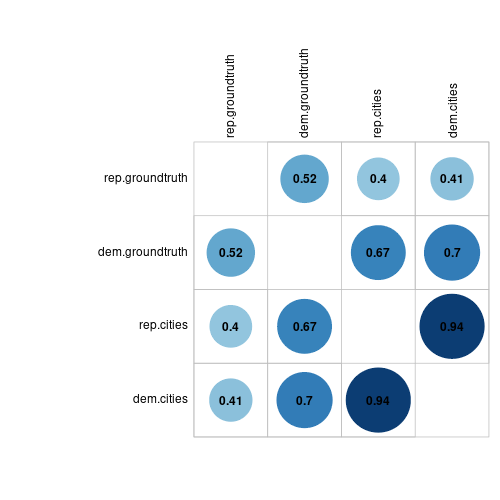
\includegraphics[width=\linewidth]{figures/groundtruth_corrplot.png}
%    \caption{Ground truth test. The values are cosine similarities between a pair of document collections.}
%    \label{groundtruth}
%\end{figure}
%
%%ground truth test
%\begin{figure}[htp]
%    \centering % Using \begin{figure*} makes the figure take up the entire width of the page
%    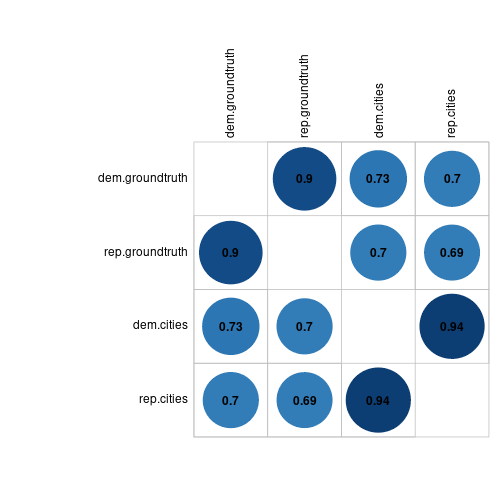
\includegraphics[width=\linewidth]{figures/groundtruth_bs_bigcities_corrplot.png}
%    \caption{Ground truth test. The values are cosine similarities between a pair of document collections (top 100 mayors vs. IN and LA).}
%    \label{groundtruth}
%\end{figure}

%Ground truth test between top100 mayors and IN + LA; with bootstrapped confidence bounds
% label: groundtruth_bootstrapped
%% latex table generated in R 3.4.3 by xtable 1.8-2 package
% Tue Feb 13 10:36:40 2018
\begin{table}[ht]
\centering
\begin{tabular}{rllll}
  \hline
 & dem.groundtruth & rep.groundtruth & dem.cities & rep.cities \\ 
  \hline
dem.groundtruth & 1, 1 & 0.807, 0.896 & 0.714, 0.729 & 0.68, 0.698 \\ 
  rep.groundtruth & 0.807, 0.896 & 1, 1 & 0.647, 0.697 & 0.641, 0.693 \\ 
  dem.cities & 0.714, 0.729 & 0.647, 0.697 & 1, 1 & 0.937, 0.944 \\ 
  rep.cities & 0.68, 0.698 & 0.641, 0.693 & 0.937, 0.944 & 1, 1 \\ 
   \hline
\end{tabular}
\caption{Ground truth test, comparing campaign websites of mayors of the 100 largest cities in the US and cities in Indiana and Louisiana. The values are bootstrapped confidence bounds for cosine similarities between concatenated document collections.} 
\label{groundtruth_bootstrapped}
\end{table}




%% latex table generated in R 3.4.4 by xtable 1.8-2 package
% Mon Apr 23 14:12:56 2018
\begin{table}[ht]
\centering
\begingroup\scriptsize
\begin{tabular}{lllllll}
  \hline
1 & 2 & 3 & 4 & 5 & 6 & 7 \\ 
  \hline
\cellcolor{red!10}yon & \cellcolor{red!10}borough & \cellcolor{red!10}port & \cellcolor{red!10}waterfront & \cellcolor{red!10}queens & \cellcolor{red!10}boroughs & \cellcolor{red!10}island \\ 
  \cellcolor{blue!10}noise & \cellcolor{blue!10}impacts & \cellcolor{blue!10}mitigation & \cellcolor{blue!10}vibration & \cellcolor{blue!10}ambient & \cellcolor{blue!10}adverse & \cellcolor{blue!10}thresholds \\ 
  \cellcolor{red!10}tax & \cellcolor{red!10}exemption & \cellcolor{red!10}taxes & \cellcolor{red!10}estate & \cellcolor{red!10}assessed & \cellcolor{red!10}real & \cellcolor{red!10}taxpayer \\ 
  \cellcolor{red!10}para & \cellcolor{red!10}personas & \cellcolor{red!10}antes & \cellcolor{red!10}persona & \cellcolor{red!10}horas & \cellcolor{red!10}junta & \cellcolor{red!10}con \\ 
  \cellcolor{blue!10}election & \cellcolor{blue!10}ethics & \cellcolor{blue!10}appointed & \cellcolor{blue!10}elections & \cellcolor{blue!10}ballot & \cellcolor{blue!10}charter & \cellcolor{blue!10}elected \\ 
  \cellcolor{red!10}wetland & \cellcolor{red!10}habitats & \cellcolor{red!10}riparian & \cellcolor{red!10}habitat & \cellcolor{red!10}wetlands & \cellcolor{red!10}tidal & \cellcolor{red!10}freshwater \\ 
  \cellcolor{blue!10}parking & \cellcolor{blue!10}bus & \cellcolor{blue!10}transit & \cellcolor{blue!10}mall & \cellcolor{blue!10}buses & \cellcolor{blue!10}campus & \cellcolor{blue!10}arena \\ 
  \cellcolor{red!30}click & \cellcolor{red!30}download & \cellcolor{red!30}online & \cellcolor{red!30}please & \cellcolor{red!30}email & \cellcolor{red!30}website & \cellcolor{red!30}visit \\ 
  \cellcolor{blue!10}draft & \cellcolor{blue!10}comments & \cellcolor{blue!10}comment & \cellcolor{blue!10}meetings & \cellcolor{blue!10}update & \cellcolor{blue!10}presentation & \cellcolor{blue!10}briefing \\ 
  \cellcolor{blue!10}ave & \cellcolor{blue!10}blvd & \cellcolor{blue!10}glen & \cellcolor{blue!10}pkwy & \cellcolor{blue!10}hwy & \cellcolor{blue!10}cove & \cellcolor{blue!10}fwy \\ 
  \cellcolor{blue!20}neighborhoods & \cellcolor{blue!20}strategy & \cellcolor{blue!20}vision & \cellcolor{blue!20}strategies & \cellcolor{blue!20}businesses & \cellcolor{blue!20}opportunities & \cellcolor{blue!20}vibrant \\ 
  \cellcolor{white}bid & \cellcolor{white}contract & \cellcolor{white}invoices & \cellcolor{white}procurement & \cellcolor{white}purchasing & \cellcolor{white}bids & \cellcolor{white}vendor \\ 
  \cellcolor{white}marijuana & \cellcolor{white}cannabis & \cellcolor{white}licensee & \cellcolor{white}taxicab & \cellcolor{white}license & \cellcolor{white}mischief & \cellcolor{white}citation \\ 
  \cellcolor{blue!10}complaint & \cellcolor{blue!10}discrimination & \cellcolor{blue!10}defendants & \cellcolor{blue!10}bankruptcy & \cellcolor{blue!10}trial & \cellcolor{blue!10}harassment & \cellcolor{blue!10}defendant \\ 
  \cellcolor{red!10}rouge & \cellcolor{red!10}baton & \cellcolor{red!10}foods & \cellcolor{red!10}parish & \cellcolor{red!10}vegetables & \cellcolor{red!10}vending & \cellcolor{red!10}cooked \\ 
  \cellcolor{red!10}child & \cellcolor{red!10}violence & \cellcolor{red!10}abuse & \cellcolor{red!10}mental & \cellcolor{red!10}clients & \cellcolor{red!10}inmates & \cellcolor{red!10}homelessness \\ 
  \cellcolor{red!10}applicants & \cellcolor{red!10}landlord & \cellcolor{red!10}tenant & \cellcolor{red!10}rent & \cellcolor{red!10}exam & \cellcolor{red!10}tenants & \cellcolor{red!10}applications \\ 
  \cellcolor{red!10}think & \cellcolor{red!10}say & \cellcolor{red!10}really & \cellcolor{red!10}thing & \cellcolor{red!10}okay & \cellcolor{red!10}got & \cellcolor{red!10}maybe \\ 
  \cellcolor{blue!20}setback & \cellcolor{blue!20}fence & \cellcolor{blue!20}yard & \cellcolor{blue!20}zoned & \cellcolor{blue!20}front & \cellcolor{blue!20}height & \cellcolor{blue!20}accessory \\ 
  \cellcolor{red!10}shall & \cellcolor{red!10}subsection & \cellcolor{red!10}article & \cellcolor{red!10}provisions & \cellcolor{red!10}pursuant & \cellcolor{red!10}thereof & \cellcolor{red!10}forth \\ 
  \cellcolor{red!20}explained & \cellcolor{red!20}asked & \cellcolor{red!20}said & \cellcolor{red!20}legislator & \cellcolor{red!20}commented & \cellcolor{red!20}advised & \cellcolor{red!20}leg \\ 
  \cellcolor{blue!10}respondents & \cellcolor{blue!10}census & \cellcolor{blue!10}population & \cellcolor{blue!10}compared & \cellcolor{blue!10}average & \cellcolor{blue!10}trends & \cellcolor{blue!10}comparison \\ 
  \cellcolor{red!20}infection & \cellcolor{red!20}symptoms & \cellcolor{red!20}breastfeeding & \cellcolor{red!20}syphilis & \cellcolor{red!20}doses & \cellcolor{red!20}asthma & \cellcolor{red!20}tuberculosis \\ 
  \cellcolor{red!20}yes & \cellcolor{red!20}name & \cellcolor{red!20}signature & \cellcolor{red!20}mailing & \cellcolor{red!20}zip & \cellcolor{red!20}attach & \cellcolor{red!20}form \\ 
  \cellcolor{red!30}games & \cellcolor{red!30}tournament & \cellcolor{red!30}swim & \cellcolor{red!30}players & \cellcolor{red!30}player & \cellcolor{red!30}camp & \cellcolor{red!30}game \\ 
  \cellcolor{blue!10}goals & \cellcolor{blue!10}implementation & \cellcolor{blue!10}policies & \cellcolor{blue!10}policy & \cellcolor{blue!10}specific & \cellcolor{blue!10}implement & \cellcolor{blue!10}comprehensive \\ 
  \cellcolor{red!20}ems & \cellcolor{red!20}fires & \cellcolor{red!20}preparedness & \cellcolor{red!20}disaster & \cellcolor{red!20}evacuation & \cellcolor{red!20}fire & \cellcolor{red!20}firefighters \\ 
  \cellcolor{red!10}subcontractor & \cellcolor{red!10}subcontractors & \cellcolor{red!10}agrees & \cellcolor{red!10}proposer & \cellcolor{red!10}contractor & \cellcolor{red!10}grantee & \cellcolor{red!10}breach \\ 
  \cellcolor{blue!10}realm & \cellcolor{blue!10}massing & \cellcolor{blue!10}facades & \cellcolor{blue!10}entrances & \cellcolor{blue!10}plazas & \cellcolor{blue!10}elements & \cellcolor{blue!10}proponents \\ 
  \cellcolor{blue!10}employee & \cellcolor{blue!10}allegation & \cellcolor{blue!10}overtime & \cellcolor{blue!10}named & \cellcolor{blue!10}leave & \cellcolor{blue!10}grievance & \cellcolor{blue!10}wage \\ 
  \cellcolor{blue!10}parks & \cellcolor{blue!10}playground & \cellcolor{blue!10}beach & \cellcolor{blue!10}park & \cellcolor{blue!10}picnic & \cellcolor{blue!10}marina & \cellcolor{blue!10}trails \\ 
  \cellcolor{blue!10}lanes & \cellcolor{blue!10}bicycle & \cellcolor{blue!10}bike & \cellcolor{blue!10}intersections & \cellcolor{blue!10}bicyclists & \cellcolor{blue!10}roadway & \cellcolor{blue!10}pedestrians \\ 
  \cellcolor{blue!20}absent & \cellcolor{blue!20}aye & \cellcolor{blue!20}khan & \cellcolor{blue!20}voting & \cellcolor{blue!20}berry & \cellcolor{blue!20}nays & \cellcolor{blue!20}tagged \\ 
  \cellcolor{blue!20}budget & \cellcolor{blue!20}revenue & \cellcolor{blue!20}million & \cellcolor{blue!20}revenues & \cellcolor{blue!20}budgeted & \cellcolor{blue!20}fund & \cellcolor{blue!20}expenditures \\ 
  \cellcolor{blue!10}whereas & \cellcolor{blue!10}resolution & \cellcolor{blue!10}amending & \cellcolor{blue!10}resolved & \cellcolor{blue!10}hereby & \cellcolor{blue!10}authorizes & \cellcolor{blue!10}digest \\ 
  \cellcolor{blue!10}assets & \cellcolor{blue!10}statements & \cellcolor{blue!10}governmental & \cellcolor{blue!10}accounting & \cellcolor{blue!10}liabilities & \cellcolor{blue!10}net & \cellcolor{blue!10}financial \\ 
  \cellcolor{red!30}honored & \cellcolor{red!30}joined & \cellcolor{red!30}proud & \cellcolor{red!30}fort & \cellcolor{red!30}announces & \cellcolor{red!30}won & \cellcolor{red!30}worth \\ 
  \cellcolor{white}analyst & \cellcolor{white}technician & \cellcolor{white}specialist & \cellcolor{white}performs & \cellcolor{white}prepares & \cellcolor{white}coordinates & \cellcolor{white}assists \\ 
  \cellcolor{white}server & \cellcolor{white}wireless & \cellcolor{white}software & \cellcolor{white}aircraft & \cellcolor{white}servers & \cellcolor{white}airport & \cellcolor{white}technology \\ 
  \cellcolor{blue!10}improvements & \cellcolor{blue!10}project & \cellcolor{blue!10}projects & \cellcolor{blue!10}phase & \cellcolor{blue!10}replacement & \cellcolor{blue!10}reconstruction & \cellcolor{blue!10}upgrades \\ 
  \cellcolor{red!10}recycling & \cellcolor{red!10}recycle & \cellcolor{red!10}garbage & \cellcolor{red!10}bags & \cellcolor{red!10}waste & \cellcolor{red!10}recyclable & \cellcolor{red!10}recyclables \\ 
  \cellcolor{blue!10}housing & \cellcolor{blue!10}affordable & \cellcolor{blue!10}households & \cellcolor{blue!10}affordability & \cellcolor{blue!10}income & \cellcolor{blue!10}moderate & \cellcolor{blue!10}homeless \\ 
  \cellcolor{red!20}effluent & \cellcolor{red!20}wastewater & \cellcolor{red!20}discharges & \cellcolor{red!20}contaminants & \cellcolor{red!20}sludge & \cellcolor{red!20}infiltration & \cellcolor{red!20}solids \\ 
  \cellcolor{red!10}fee & \cellcolor{red!10}permit & \cellcolor{red!10}inspection & \cellcolor{red!10}permits & \cellcolor{red!10}inspections & \cellcolor{red!10}fees & \cellcolor{red!10}occupancy \\ 
  \cellcolor{blue!10}uses & \cellcolor{blue!10}mixed & \cellcolor{blue!10}density & \cellcolor{blue!10}land & \cellcolor{blue!10}industrial & \cellcolor{blue!10}residential & \cellcolor{blue!10}commercial \\ 
  \cellcolor{red!10}energy & \cellcolor{red!10}renewable & \cellcolor{red!10}coal & \cellcolor{red!10}electricity & \cellcolor{red!10}climate & \cellcolor{red!10}solar & \cellcolor{red!10}greenhouse \\ 
  \cellcolor{blue!10}bonds & \cellcolor{blue!10}refunding & \cellcolor{blue!10}securities & \cellcolor{blue!10}bond & \cellcolor{blue!10}debt & \cellcolor{blue!10}issuer & \cellcolor{blue!10}maturity \\ 
  \cellcolor{red!20}artists & \cellcolor{red!20}artist & \cellcolor{red!20}performances & \cellcolor{red!20}music & \cellcolor{red!20}orchestra & \cellcolor{red!20}symphony & \cellcolor{red!20}arts \\ 
  \cellcolor{blue!80}arrested & \cellcolor{blue!80}suspect & \cellcolor{blue!80}homicide & \cellcolor{blue!80}suspects & \cellcolor{blue!80}shooting & \cellcolor{blue!80}sergeant & \cellcolor{blue!80}arrests \\ 
  \cellcolor{white}retiree & \cellcolor{white}actuarial & \cellcolor{white}retirement & \cellcolor{white}deductible & \cellcolor{white}retirees & \cellcolor{white}copay & \cellcolor{white}dental \\ 
  \cellcolor{red!10}ferrets & \cellcolor{red!10}dogs & \cellcolor{red!10}cats & \cellcolor{red!10}rabies & \cellcolor{red!10}pets & \cellcolor{red!10}spay & \cellcolor{red!10}stray \\ 
  \cellcolor{blue!10}audit & \cellcolor{blue!10}auditor & \cellcolor{blue!10}audits & \cellcolor{blue!10}procedures & \cellcolor{blue!10}controls & \cellcolor{blue!10}implemented & \cellcolor{blue!10}accountability \\ 
  \cellcolor{blue!10}avenue & \cellcolor{blue!10}west & \cellcolor{blue!10}east & \cellcolor{blue!10}south & \cellcolor{blue!10}north & \cellcolor{blue!10}thence & \cellcolor{blue!10}street \\ 
  \cellcolor{white}historic & \cellcolor{white}revival & \cellcolor{white}landmarks & \cellcolor{white}landmark & \cellcolor{white}craftsman & \cellcolor{white}bungalow & \cellcolor{white}style \\ 
  \cellcolor{red!10}remodel & \cellcolor{red!10}monoxide & \cellcolor{red!10}alarms & \cellcolor{red!10}roofing & \cellcolor{red!10}heater & \cellcolor{red!10}description & \cellcolor{red!10}bathroom \\ 
  \cellcolor{red!10}motion & \cellcolor{red!10}alderman & \cellcolor{red!10}seconded & \cellcolor{red!10}carried & \cellcolor{red!10}whiting & \cellcolor{red!10}unanimously & \cellcolor{red!10}ayes \\ 
  \cellcolor{white}pruning & \cellcolor{white}tree & \cellcolor{white}forestry & \cellcolor{white}trees & \cellcolor{white}mulch & \cellcolor{white}planting & \cellcolor{white}planted \\ 
  \cellcolor{red!10}fittings & \cellcolor{red!10}joints & \cellcolor{red!10}thickness & \cellcolor{red!10}pipe & \cellcolor{red!10}trench & \cellcolor{red!10}valve & \cellcolor{red!10}psi \\ 
  \cellcolor{white}students & \cellcolor{white}learning & \cellcolor{white}schools & \cellcolor{white}student & \cellcolor{white}academic & \cellcolor{white}career & \cellcolor{white}education \\ 
  \cellcolor{red!20}plat & \cellcolor{red!20}sign & \cellcolor{red!20}pud & \cellcolor{red!20}petitioner & \cellcolor{red!20}petition & \cellcolor{red!20}variance & \cellcolor{red!20}subdivision \\ 
   \hline
\end{tabular}
\endgroup
\caption{Top words from a structural topic model with 60 topics and FREX scoring. Colors depict partisanship based on coefficient size. White cells are non-significant topics. Based on data preprocessed without the classifier.} 
\end{table}

 %\ref{tabSTMtopwords}


% latex table generated in R 3.4.4 by xtable 1.8-2 package
% Fri Aug 10 15:33:35 2018
\begin{table}[ht]
\centering
\begingroup\footnotesize
\begin{tabular}{rllllllll}
  \hline
 \# & Top Word 1 & Top Word 2 & Top Word 3 & Top Word 4 & Top Word 5 & Top Word 6 & \multicolumn{2}{c}{Tokens assigned} \\ 
  \hline
   42 & \cellcolor{red!20}breastfeed & \cellcolor{red!20}vaccine & \cellcolor{red!20}infection & \cellcolor{red!20}symptom & \cellcolor{red!20}asthma & \cellcolor{red!20}mosquito & \mybar{2497} \\ 
   17 & \cellcolor{red!20}alarm & \cellcolor{red!20}disaster & \cellcolor{red!20}fire & \cellcolor{red!20}rescue & \cellcolor{red!20}preparedness & \cellcolor{red!20}evacuation & \mybar{989} \\ 
   53 & \cellcolor{red!20}drinking & \cellcolor{red!20}wastewater & \cellcolor{red!20}water & \cellcolor{red!20}pipeline & \cellcolor{red!20}pump & \cellcolor{red!20}disinfection & \mybar{461} \\ 

   49 & \cellcolor{red!10}bin & \cellcolor{red!10}recycling & \cellcolor{red!10}garbage & \cellcolor{red!10}recyclables & \cellcolor{red!10}recyclable & \cellcolor{red!10}bag & \mybar{1791} \\ 
    7 & \cellcolor{red!10}energy & \cellcolor{red!10}garland & \cellcolor{red!10}renewable & \cellcolor{red!10}solar & \cellcolor{red!10}electricity & \cellcolor{red!10}climate & \mybar{742} \\ 
   23 & \cellcolor{red!10}bid & \cellcolor{red!10}proposer & \cellcolor{red!10}bidder & \cellcolor{red!10}contractor & \cellcolor{red!10}subcontractor & \cellcolor{red!10}contract & \mybar{447} \\ 
   57 & \cellcolor{red!10}duct & \cellcolor{red!10}conduit & \cellcolor{red!10}bolt & \cellcolor{red!10}splice & \cellcolor{red!10}valve & \cellcolor{red!10}fitting & \mybar{1373} \\ 
   13 & \cellcolor{red!10}server & \cellcolor{red!10}wireless & \cellcolor{red!10}software & \cellcolor{red!10}telecommunication & \cellcolor{red!10}subscriber & \cellcolor{red!10}desktop & \mybar{1092} \\ 
    1 & \cellcolor{red!10}storm & \cellcolor{red!10}runoff & \cellcolor{red!10}infiltration & \cellcolor{red!10}discharge & \cellcolor{red!10}drainage & \cellcolor{red!10}drain & \mybar{516} \\ 
   38 & \cellcolor{red!10}youth & \cellcolor{red!10}student & \cellcolor{red!10}parent & \cellcolor{red!10}teacher & \cellcolor{red!10}immigrant & \cellcolor{red!10}literacy & \mybar{714} \\ 
   59 & \cellcolor{red!10}sampling & \cellcolor{red!10}sample & \cellcolor{red!10}analytical & \cellcolor{red!10}concentration & \cellcolor{red!10}hydrocarbon & \cellcolor{red!10}toxicity & \mybar{1241} \\ 
   45 & \cellcolor{red!10}premise & \cellcolor{red!10}licensee & \cellcolor{red!10}violation & \cellcolor{red!10}license & \cellcolor{red!10}permit & \cellcolor{red!10}inspection & \mybar{509} \\ 
   60 & \cellcolor{red!10}exhaust & \cellcolor{red!10}fugitive & \cellcolor{red!10}aircraft & \cellcolor{red!10}airport & \cellcolor{red!10}aviation & \cellcolor{red!10}diesel & \mybar{731} \\ 
   %30 & \cellcolor{white}fort & \cellcolor{white}thence & \cellcolor{white}blvd & \cellcolor{white}worth & \cellcolor{white}ave & \cellcolor{white}west & \mybar{681} \\ 
   %58 & \cellcolor{white}councilor & \cellcolor{white}auburn & \cellcolor{white}plain & \cellcolor{white}ward & \cellcolor{white}beech & \cellcolor{white}glen & \mybar{480} \\ 
   %51 & \cellcolor{white}whereas & \cellcolor{white}councilman & \cellcolor{white}alderman & \cellcolor{white}ordain & \cellcolor{white}hereby & \cellcolor{white}resolution & \mybar{420} \\ 
   %16 & \cellcolor{white}recreation & \cellcolor{white}park & \cellcolor{white}golf & \cellcolor{white}playground & \cellcolor{white}picnic & \cellcolor{white}zoo & \mybar{682} \\ 
   %36 & \cellcolor{white}retiree & \cellcolor{white}retirement & \cellcolor{white}actuarial & \cellcolor{white}deductible & \cellcolor{white}dental & \cellcolor{white}pension & \mybar{470} \\ 
   %27 & \cellcolor{white}exam & \cellcolor{white}incumbent & \cellcolor{white}supervise & \cellcolor{white}supervision & \cellcolor{white}examination & \cellcolor{white}knowledge & \mybar{687} \\ 
   %56 & \cellcolor{white}historic & \cellcolor{white}landmark & \cellcolor{white}revival & \cellcolor{white}archaeological & \cellcolor{white}century & \cellcolor{white}historian & \mybar{2587} \\ 
   %12 & \cellcolor{white}parking & \cellcolor{white}hotel & \cellcolor{white}garage & \cellcolor{white}space & \cellcolor{white}retail & \cellcolor{white}square & \mybar{321} \\ 
   %41 & \cellcolor{white}tax & \cellcolor{white}exemption & \cellcolor{white}abatement & \cellcolor{white}real & \cellcolor{white}estate & \cellcolor{white}property & \mybar{310} \\ 
    4 & \cellcolor{white}facade & \cellcolor{white}awning & \cellcolor{white}porch & \cellcolor{white}roof & \cellcolor{white}balcony & \cellcolor{white}exterior & \mybar{1108} \\ 

   15 & \cellcolor{blue!10}complainant & \cellcolor{blue!10}defendant & \cellcolor{blue!10}allegation & \cellcolor{blue!10}complaint & \cellcolor{blue!10}allege & \cellcolor{blue!10}discrimination & \mybar{1384} \\ 
 
   14 & \cellcolor{blue!10}yes & \cellcolor{blue!10}agency & \cellcolor{blue!10}federal & \cellcolor{blue!10}recipient & \cellcolor{blue!10}compliance & \cellcolor{blue!10}entity & \mybar{205} \\ 

   25 & \cellcolor{blue!10}cannabis & \cellcolor{blue!10}marijuana & \cellcolor{blue!10}senate & \cellcolor{blue!10}dispensary & \cellcolor{blue!10}ballot & \cellcolor{blue!10}cultivation & \mybar{1188} \\ 

   47 & \cellcolor{blue!10}employee & \cellcolor{blue!10}overtime & \cellcolor{blue!10}sick & \cellcolor{blue!10}wage & \cellcolor{blue!10}grievance & \cellcolor{blue!10}bargaining & \mybar{511} \\ 

   37 & \cellcolor{blue!10}audit & \cellcolor{blue!10}auditor & \cellcolor{blue!10}internal & \cellcolor{blue!10}procedure & \cellcolor{blue!10}accountability & \cellcolor{blue!10}oversight & \mybar{420} \\ 
   21 & \cellcolor{blue!10}housing & \cellcolor{blue!10}affordable & \cellcolor{blue!10}homeless & \cellcolor{blue!10}homelessness & \cellcolor{blue!10}affordability & \cellcolor{blue!10}landlord & \mybar{318} \\ 
   34 & \cellcolor{blue!10}comment & \cellcolor{blue!10}draft & \cellcolor{blue!10}feedback & \cellcolor{blue!10}stakeholder & \cellcolor{blue!10}suggest & \cellcolor{blue!10}discussion & \mybar{289} \\ 
   19 & \cellcolor{blue!10}debt & \cellcolor{blue!10}bond & \cellcolor{blue!10}governmental & \cellcolor{blue!10}obligation & \cellcolor{blue!10}financial & \cellcolor{blue!10}accounting & \mybar{251} \\ 
   40 & \cellcolor{blue!10}bicycle & \cellcolor{blue!10}bike & \cellcolor{blue!10}lane & \cellcolor{blue!10}crosswalk & \cellcolor{blue!10}pedestrian & \cellcolor{blue!10}bicyclist & \mybar{574} \\ 
   32 & \cellcolor{blue!20}budget & \cellcolor{blue!20}revenue & \cellcolor{blue!20}expenditure & \cellcolor{blue!20}appropriation & \cellcolor{blue!20}fund & \cellcolor{blue!20}million & \mybar{242} \\ 
   48 & \cellcolor{blue!20}absent & \cellcolor{blue!20}aye & \cellcolor{blue!20}khan & \cellcolor{blue!20}nay & \cellcolor{blue!20}berry & \cellcolor{blue!20}voting & \mybar{528} \\ 
   31 & \cellcolor{blue!20}chair & \cellcolor{blue!20}agenda & \cellcolor{blue!20}commission & \cellcolor{blue!20}speaker & \cellcolor{blue!20}chairperson & \cellcolor{blue!20}committee & \mybar{314} \\ 
   55 & \cellcolor{blue!80}robbery & \cellcolor{blue!80}homicide & \cellcolor{blue!80}arrest & \cellcolor{blue!80}sergeant & \cellcolor{blue!80}suspect & \cellcolor{blue!80}burglary & \mybar{1395} \\ 
   \hline
\end{tabular}
\endgroup
%\caption{Top words from a structural topic model with 60 topics and FREX scoring. Colors depict partisanship based on coefficient size. White cells are non-significant topics.} 
\label{tabSTMtopwords60}
\end{table}


%% latex table generated in R 3.4.4 by xtable 1.8-2 package
% Fri Aug 10 15:33:35 2018
\begin{table}[ht]
\centering
\begingroup\scriptsize
\begin{tabular}{rllllllll}
  \hline
 \# & Top Word 1 & Top Word 2 & Top Word 3 & Top Word 4 & Top Word 5 & Top Word 6 & \multicolumn{2}{c}{Tokens assigned} \\ 
  \hline
 43 & \cellcolor{red!50}fun & \cellcolor{red!50}player & \cellcolor{red!50}dream & \cellcolor{red!50}celebration & \cellcolor{red!50}favorite & \cellcolor{red!50}blog & \mybar{3460} \\ 
    5 & \cellcolor{red!30}please & \cellcolor{red!30}email & \cellcolor{red!30}contact & \cellcolor{red!30}copy & \cellcolor{red!30}mail & \cellcolor{red!30}click & \mybar{201} \\ 
   42 & \cellcolor{red!20}breastfeed & \cellcolor{red!20}vaccine & \cellcolor{red!20}infection & \cellcolor{red!20}symptom & \cellcolor{red!20}asthma & \cellcolor{red!20}mosquito & \mybar{2497} \\ 
   17 & \cellcolor{red!20}alarm & \cellcolor{red!20}disaster & \cellcolor{red!20}fire & \cellcolor{red!20}rescue & \cellcolor{red!20}preparedness & \cellcolor{red!20}evacuation & \mybar{989} \\ 
   53 & \cellcolor{red!20}drinking & \cellcolor{red!20}wastewater & \cellcolor{red!20}water & \cellcolor{red!20}pipeline & \cellcolor{red!20}pump & \cellcolor{red!20}disinfection & \mybar{461} \\ 
   50 & \cellcolor{red!20}buffalo & \cellcolor{red!20}news & \cellcolor{red!20}honor & \cellcolor{red!20}warren & \cellcolor{red!20}announce & \cellcolor{red!20}lovely & \mybar{1106} \\ 
   52 & \cellcolor{red!20}reappoints & \cellcolor{red!20}digest & \cellcolor{red!20}cat & \cellcolor{red!20}leg & \cellcolor{red!20}legislator & \cellcolor{red!20}sander & \mybar{997} \\ 
   33 & \cellcolor{red!20}really & \cellcolor{red!20}think & \cellcolor{red!20}something & \cellcolor{red!20}thing & \cellcolor{red!20}somebody & \cellcolor{red!20}anybody & \mybar{1873} \\ 
   44 & \cellcolor{red!10}shall & \cellcolor{red!10}herein & \cellcolor{red!10}forth & \cellcolor{red!10}deem & \cellcolor{red!10}thereof & \cellcolor{red!10}pursuant & \mybar{405} \\ 
    8 & \cellcolor{red!10}invoice & \cellcolor{red!10}card & \cellcolor{red!10}amt & \cellcolor{red!10}filer & \cellcolor{red!10}debit & \cellcolor{red!10}officeholder & \mybar{527} \\ 
   26 & \cellcolor{red!10}fee & \cellcolor{red!10}charge & \cellcolor{red!10}billing & \cellcolor{red!10}per & \cellcolor{red!10}meter & \cellcolor{red!10}monthly & \mybar{233} \\ 
    2 & \cellcolor{red!10}yon & \cellcolor{red!10}borough & \cellcolor{red!10}comm & \cellcolor{red!10}gen & \cellcolor{red!10}sou & \cellcolor{red!10}spec & \mybar{709} \\ 
   49 & \cellcolor{red!10}bin & \cellcolor{red!10}recycling & \cellcolor{red!10}garbage & \cellcolor{red!10}recyclables & \cellcolor{red!10}recyclable & \cellcolor{red!10}bag & \mybar{1791} \\ 
    7 & \cellcolor{red!10}energy & \cellcolor{red!10}garland & \cellcolor{red!10}renewable & \cellcolor{red!10}solar & \cellcolor{red!10}electricity & \cellcolor{red!10}climate & \mybar{742} \\ 
   23 & \cellcolor{red!10}bid & \cellcolor{red!10}proposer & \cellcolor{red!10}bidder & \cellcolor{red!10}contractor & \cellcolor{red!10}subcontractor & \cellcolor{red!10}contract & \mybar{447} \\ 
   57 & \cellcolor{red!10}duct & \cellcolor{red!10}conduit & \cellcolor{red!10}bolt & \cellcolor{red!10}splice & \cellcolor{red!10}valve & \cellcolor{red!10}fitting & \mybar{1373} \\ 
   13 & \cellcolor{red!10}server & \cellcolor{red!10}wireless & \cellcolor{red!10}software & \cellcolor{red!10}telecommunication & \cellcolor{red!10}subscriber & \cellcolor{red!10}desktop & \mybar{1092} \\ 
   54 & \cellcolor{red!10}motion & \cellcolor{red!10}adjourn & \cellcolor{red!10}second & \cellcolor{red!10}unanimously & \cellcolor{red!10}ayes & \cellcolor{red!10}carry & \mybar{474} \\ 
    1 & \cellcolor{red!10}storm & \cellcolor{red!10}runoff & \cellcolor{red!10}infiltration & \cellcolor{red!10}discharge & \cellcolor{red!10}drainage & \cellcolor{red!10}drain & \mybar{516} \\ 
   38 & \cellcolor{red!10}youth & \cellcolor{red!10}student & \cellcolor{red!10}parent & \cellcolor{red!10}teacher & \cellcolor{red!10}immigrant & \cellcolor{red!10}literacy & \mybar{714} \\ 
   35 & \cellcolor{red!10}artist & \cellcolor{red!10}rouge & \cellcolor{red!10}baton & \cellcolor{red!10}art & \cellcolor{red!10}artwork & \cellcolor{red!10}exhibition & \mybar{1632} \\ 
   59 & \cellcolor{red!10}sampling & \cellcolor{red!10}sample & \cellcolor{red!10}analytical & \cellcolor{red!10}concentration & \cellcolor{red!10}hydrocarbon & \cellcolor{red!10}toxicity & \mybar{1241} \\ 
    3 & \cellcolor{red!10}portfolio & \cellcolor{red!10}yield & \cellcolor{red!10}jun & \cellcolor{red!10}maturity & \cellcolor{red!10}investment & \cellcolor{red!10}rating & \mybar{544} \\ 
   45 & \cellcolor{red!10}premise & \cellcolor{red!10}licensee & \cellcolor{red!10}violation & \cellcolor{red!10}license & \cellcolor{red!10}permit & \cellcolor{red!10}inspection & \mybar{509} \\ 
    9 & \cellcolor{red!10}para & \cellcolor{red!10}persona & \cellcolor{red!10}ante & \cellcolor{red!10}horas & \cellcolor{red!10}junta & \cellcolor{red!10}largo & \mybar{1469} \\ 
   60 & \cellcolor{red!10}exhaust & \cellcolor{red!10}fugitive & \cellcolor{red!10}aircraft & \cellcolor{red!10}airport & \cellcolor{red!10}aviation & \cellcolor{red!10}diesel & \mybar{731} \\ 
   30 & \cellcolor{white}fort & \cellcolor{white}thence & \cellcolor{white}blvd & \cellcolor{white}worth & \cellcolor{white}ave & \cellcolor{white}west & \mybar{681} \\ 
   58 & \cellcolor{white}councilor & \cellcolor{white}auburn & \cellcolor{white}plain & \cellcolor{white}ward & \cellcolor{white}beech & \cellcolor{white}glen & \mybar{480} \\ 
   51 & \cellcolor{white}whereas & \cellcolor{white}councilman & \cellcolor{white}alderman & \cellcolor{white}ordain & \cellcolor{white}hereby & \cellcolor{white}resolution & \mybar{420} \\ 
   16 & \cellcolor{white}recreation & \cellcolor{white}park & \cellcolor{white}golf & \cellcolor{white}playground & \cellcolor{white}picnic & \cellcolor{white}zoo & \mybar{682} \\ 
   36 & \cellcolor{white}retiree & \cellcolor{white}retirement & \cellcolor{white}actuarial & \cellcolor{white}deductible & \cellcolor{white}dental & \cellcolor{white}pension & \mybar{470} \\ 
   27 & \cellcolor{white}exam & \cellcolor{white}incumbent & \cellcolor{white}supervise & \cellcolor{white}supervision & \cellcolor{white}examination & \cellcolor{white}knowledge & \mybar{687} \\ 
   56 & \cellcolor{white}historic & \cellcolor{white}landmark & \cellcolor{white}revival & \cellcolor{white}archaeological & \cellcolor{white}century & \cellcolor{white}historian & \mybar{2587} \\ 
   12 & \cellcolor{white}parking & \cellcolor{white}hotel & \cellcolor{white}garage & \cellcolor{white}space & \cellcolor{white}retail & \cellcolor{white}square & \mybar{321} \\ 
   41 & \cellcolor{white}tax & \cellcolor{white}exemption & \cellcolor{white}abatement & \cellcolor{white}real & \cellcolor{white}estate & \cellcolor{white}property & \mybar{310} \\ 
    4 & \cellcolor{white}facade & \cellcolor{white}awning & \cellcolor{white}porch & \cellcolor{white}roof & \cellcolor{white}balcony & \cellcolor{white}exterior & \mybar{1108} \\ 
   28 & \cellcolor{blue!10}census & \cellcolor{blue!10}population & \cellcolor{blue!10}respondent & \cellcolor{blue!10}figure & \cellcolor{blue!10}percent & \cellcolor{blue!10}margin & \mybar{541} \\ 
   18 & \cellcolor{blue!10}prune & \cellcolor{blue!10}tree & \cellcolor{blue!10}deer & \cellcolor{blue!10}forestry & \cellcolor{blue!10}shrub & \cellcolor{blue!10}bulrush & \mybar{2522} \\ 
   15 & \cellcolor{blue!10}complainant & \cellcolor{blue!10}defendant & \cellcolor{blue!10}allegation & \cellcolor{blue!10}complaint & \cellcolor{blue!10}allege & \cellcolor{blue!10}discrimination & \mybar{1384} \\ 
   20 & \cellcolor{blue!10}noise & \cellcolor{blue!10}mitigation & \cellcolor{blue!10}impact & \cellcolor{blue!10}adverse & \cellcolor{blue!10}significant & \cellcolor{blue!10}vibration & \mybar{325} \\ 
   14 & \cellcolor{blue!10}yes & \cellcolor{blue!10}agency & \cellcolor{blue!10}federal & \cellcolor{blue!10}recipient & \cellcolor{blue!10}compliance & \cellcolor{blue!10}entity & \mybar{205} \\ 
   46 & \cellcolor{blue!10}variance & \cellcolor{blue!10}setback & \cellcolor{blue!10}plat & \cellcolor{blue!10}zoning & \cellcolor{blue!10}yard & \cellcolor{blue!10}fence & \mybar{289} \\ 
   29 & \cellcolor{blue!10}learn & \cellcolor{blue!10}neighborhood & \cellcolor{blue!10}graffito & \cellcolor{blue!10}event & \cellcolor{blue!10}resident & \cellcolor{blue!10}online & \mybar{196} \\ 
   25 & \cellcolor{blue!10}cannabis & \cellcolor{blue!10}marijuana & \cellcolor{blue!10}senate & \cellcolor{blue!10}dispensary & \cellcolor{blue!10}ballot & \cellcolor{blue!10}cultivation & \mybar{1188} \\ 
   22 & \cellcolor{blue!10}priority & \cellcolor{blue!10}strategic & \cellcolor{blue!10}ongoing & \cellcolor{blue!10}goal & \cellcolor{blue!10}implementation & \cellcolor{blue!10}implement & \mybar{141} \\ 
    6 & \cellcolor{blue!10}project & \cellcolor{blue!10}improvement & \cellcolor{blue!10}phase & \cellcolor{blue!10}replacement & \cellcolor{blue!10}upgrade & \cellcolor{blue!10}capital & \mybar{174} \\ 
   11 & \cellcolor{blue!10}shoreline & \cellcolor{blue!10}beach & \cellcolor{blue!10}marina & \cellcolor{blue!10}coastal & \cellcolor{blue!10}waterfront & \cellcolor{blue!10}salmon & \mybar{1069} \\ 
   24 & \cellcolor{blue!10}attract & \cellcolor{blue!10}economy & \cellcolor{blue!10}workforce & \cellcolor{blue!10}innovation & \cellcolor{blue!10}sector & \cellcolor{blue!10}economic & \mybar{748} \\ 
   47 & \cellcolor{blue!10}employee & \cellcolor{blue!10}overtime & \cellcolor{blue!10}sick & \cellcolor{blue!10}wage & \cellcolor{blue!10}grievance & \cellcolor{blue!10}bargaining & \mybar{511} \\ 
   39 & \cellcolor{blue!10}tab & \cellcolor{blue!10}accessibility & \cellcolor{blue!10}mode & \cellcolor{blue!10}var & \cellcolor{blue!10}alt & \cellcolor{blue!10}false & \mybar{259} \\ 
   10 & \cellcolor{blue!10}density & \cellcolor{blue!10}village & \cellcolor{blue!10}urban & \cellcolor{blue!10}us & \cellcolor{blue!10}mixed & \cellcolor{blue!10}corridor & \mybar{358} \\ 
   37 & \cellcolor{blue!10}audit & \cellcolor{blue!10}auditor & \cellcolor{blue!10}internal & \cellcolor{blue!10}procedure & \cellcolor{blue!10}accountability & \cellcolor{blue!10}oversight & \mybar{420} \\ 
   21 & \cellcolor{blue!10}housing & \cellcolor{blue!10}affordable & \cellcolor{blue!10}homeless & \cellcolor{blue!10}homelessness & \cellcolor{blue!10}affordability & \cellcolor{blue!10}landlord & \mybar{318} \\ 
   34 & \cellcolor{blue!10}comment & \cellcolor{blue!10}draft & \cellcolor{blue!10}feedback & \cellcolor{blue!10}stakeholder & \cellcolor{blue!10}suggest & \cellcolor{blue!10}discussion & \mybar{289} \\ 
   19 & \cellcolor{blue!10}debt & \cellcolor{blue!10}bond & \cellcolor{blue!10}governmental & \cellcolor{blue!10}obligation & \cellcolor{blue!10}financial & \cellcolor{blue!10}accounting & \mybar{251} \\ 
   40 & \cellcolor{blue!10}bicycle & \cellcolor{blue!10}bike & \cellcolor{blue!10}lane & \cellcolor{blue!10}crosswalk & \cellcolor{blue!10}pedestrian & \cellcolor{blue!10}bicyclist & \mybar{574} \\ 
   32 & \cellcolor{blue!20}budget & \cellcolor{blue!20}revenue & \cellcolor{blue!20}expenditure & \cellcolor{blue!20}appropriation & \cellcolor{blue!20}fund & \cellcolor{blue!20}million & \mybar{242} \\ 
   48 & \cellcolor{blue!20}absent & \cellcolor{blue!20}aye & \cellcolor{blue!20}khan & \cellcolor{blue!20}nay & \cellcolor{blue!20}berry & \cellcolor{blue!20}voting & \mybar{528} \\ 
   31 & \cellcolor{blue!20}chair & \cellcolor{blue!20}agenda & \cellcolor{blue!20}commission & \cellcolor{blue!20}speaker & \cellcolor{blue!20}chairperson & \cellcolor{blue!20}committee & \mybar{314} \\ 
   55 & \cellcolor{blue!80}robbery & \cellcolor{blue!80}homicide & \cellcolor{blue!80}arrest & \cellcolor{blue!80}sergeant & \cellcolor{blue!80}suspect & \cellcolor{blue!80}burglary & \mybar{1395} \\ 
   \hline
\end{tabular}
\endgroup
\caption{OLD: Top words from a structural topic model with 60 topics and FREX scoring. Colors depict partisanship based on coefficient size. White cells are non-significant topics.} 
\label{tabSTMtopwords60}
\end{table}

 %\ref{tabSTMtopwords2}

\section{Conclusion}


We have developed a methodological pipeline for automatically gathering and preparing government websites for comparative content analysis. We have produced an R package \texttt{gov2text}, in which we have implemented and wrapped the core components of our pipeline. This methodology holds the potential to vastly scale up the data collection efforts underpinning the growing body of research that is focused on government website analysis. Through an application to the analysis of municipal websites in six different states, we show how our pipeline is capable of gathering corpora that shed light on the forms and functions of local government. We find that government website contents are associated with the partisanship of the mayor in ways that would be expected based on the parties' national priorities and past research on the effects of mayoral partisanship on city governments.

The biggest limitation in our pipeline, and an open area for future research, is the reliance on \texttt{wget} to gather the initial website files. By using \texttt{wget}, we miss content that is displayed dynamically on websites using JavaScript. For any one website, it would be possible to customize a routine with \texttt{Selenium} to access dynamic elements, but the process would need to be customized for each website.\footnote{ We investigated whether the presence of JavaScript was related to the amount of text we gathered from the website. We calculated the correlation between the number of <script> HTML tags on a city's website, which indicate the use of JavaScript on a site, and the number of text tokens we scrape from the site. This correlation is -0.059, which indicates a very weak relationship between the use of JavaScript and the amount of text scraped from the site.}

%We offer several contributions that will be valuable in future research endeavors. First, the data collected in the current study can be used for comparative analysis of US city website contents. Second, the pipeline we present can be used as a set of procedures to follow in gathering large-scale datasets of textual contents from other samples of governments. For example, the pipeline we have developed could be used to build comparative datasets of state or federal bureaucratic agencies. Third, our findings regarding the effects of mayoral partisanship on city website contents advance the literature on the role of partisan leadership in local government, and reinforce the finding of \citet{gerber2011mayors} that the effects of mayoral partisanship can be best observed through the analysis of domains of government (e.g., website contents) that are not heavily constrained by state or national governments.

\section*{Funding}
This work was supported by the National Science Foundation [1320219, 1637089, 1641047].

%% latex table generated in R 3.5.0 by xtable 1.8-2 package
% Wed Jul  4 14:14:10 2018
\begin{table}[ht]
\centering
\begin{tabular}{lrr}
  \hline
State & Democratic & Republican \\ 
  \hline
California &   9 &   6 \\ 
  Indiana &  46 &  54 \\ 
  Louisiana &  28 &  17 \\ 
  New York &  36 &  16 \\ 
  Texas &   2 &   7 \\ 
  Washington &  11 &   2 \\ 
   \hline
\end{tabular}
\caption{Descriptive statistics on the partisanship of the cities in the corpus.} 
\end{table}


%% latex table generated in R 3.4.3 by xtable 1.8-2 package
% Fri Mar  2 19:05:45 2018
\begin{table}[ht]
\centering
\begin{tabular}{lr}
  \hline
State & Cities \\ 
  \hline
Alabama &   1 \\ 
  Alaska &   1 \\ 
  Arizona &   6 \\ 
  California &  15 \\ 
  Colorado &   3 \\ 
  D.C. &   1 \\ 
  Florida &   6 \\ 
  Georgia &   1 \\ 
  Hawaii &   1 \\ 
  Idaho &   1 \\ 
  Illinois &   1 \\ 
  Indiana & 108 \\ 
  Kansas &   1 \\ 
  Kentucky &   2 \\ 
  Louisiana &  57 \\ 
  Maryland &   1 \\ 
  Massachusetts &   1 \\ 
  Michigan &   1 \\ 
  Minnesota &   2 \\ 
  Missouri &   2 \\ 
  Nebraska &   2 \\ 
  Nevada &   2 \\ 
  New Jersey &   2 \\ 
  New Mexico &   1 \\ 
  New York &  52 \\ 
  North Carolina &   4 \\ 
  Ohio &   4 \\ 
  Oklahoma &   2 \\ 
  Oregon &   1 \\ 
  Pennsylvania &   2 \\ 
  Tennessee &   2 \\ 
  Texas &  10 \\ 
  Virginia &   3 \\ 
  Washington &  13 \\ 
  Wisconsin &   2 \\ 
   \hline
\end{tabular}
\caption{Number of cities per state for which we have information about partisanship as well as the city's website URL.} 
\label{stateUrlSummary}
\end{table}



\bibliographystyle{chicago} % apsr stopped working for me
%\bibliographystyle{plainnat}
\bibliography{ref}


\end{document}



